%\begin{abstract}
%
%Within the civil violence literature there is an emerging body of research that
%stresses the potential conflict inducing effects of precolonial states. On the
%other hand, the literature on communal violence has emphasized the potential
%conflict reducing effects of local institutions associated with prior statehood.
%We address this apparent puzzle by arguing that an initial reduction of
%commitment issues and inter-group security dilemma introduced by pre-colonial
%states set in motion a positive feedback loop of increased trade, reduced
%information problems, increased relative gains from continued cooperation, and a
%legacy of mixed ethnic settlement patterns. In support of the proposed mechanism
%we find that more precolonial state presence is associated with higher levels of
%ethnic fractionalization, and while precolonial states could cause more state
%based violence we find a general conflict reducing effect on communal violence.
%This effect is particularly strong in East Africa.
%
%% Too different from the rest of the text? We don't mention this puzzle. Should
%% we?
%
%\end{abstract}
%
%\bigskip
%
%\keywords{Precolonial states, communal violence, non-state violence,
%inter-ethnic violence}
%
%\pagebreak
%
%\onehalfspacing
%
%% }}}

\chapter{Communal violence and the legacy of pre-colonial states}

The level of violence in non-state societies is qualitatively different from
that in state societies with levels often several orders magnitude higher in the
former \citep{diamond2013world, LeBlanc2003, Pinker2012}. Part of this can be
explained by the states’ role in solving the security dilemma \citep{Hobbes,
Lake_1996}. Several states in contemporary sub-Saharan Africa are judicially
sovereign, but empirically less effective \citep{Jackson_1982}. This has
resulted in pockets where the resolution of violent intergroup conflicts is
mainly left to local traditional mechanisms without a neutral arbiter to mediate
or enforce peace, should things get out of hand. There are important variations
in the extent to which states have areas without strong state control, however,
as some areas have a long precolonial legacy of statehood which have addressed
the security dilemma between social groups. Some claim that the existence of
precolonial states has caused legal ambiguities that are important causes of
intergroup violence \citep{Eck2014}, others hold that remnants of precolonial
institutions directly \citep{Herbst2014, Wig2018} or indirectly reduce the
overall number of inter-group (communal) conflicts. We argue that by having
reduced non-state violence in the past, precolonial states have left a legacy of
reduced security dilemmas and commitment problems, as well as increased
intergroup interaction and trade. In addition to continuity of traditional
institutions and more structures to build on for contemporary states, these
mechanisms continue to reduce communal violence in the areas controlled by
precolonial states to this day. In support of this argument we find a
significant and robust negative association between local levels of precolonial
state presence and local levels of communal violence. The proposed mechanisms
are supported by ethnic settlement patterns largely conforming to theoretical
expectations. Despite the evidence of a general effect, there are large regional
differences in the results. In particular, Nigeria stands out, with high levels
of communal violence in areas of substantial precolonial state presence. We
suspect these results are due to national level dynamics in inter-group
conflicts in this country, in contrast to the predominantly local character of
such conflicts elsewhere. However, more research is needed to determine when and
where different mechanisms might apply, or whether existing measures are picking
up distinct phenomenon.

\section{How conflicts are prevented or resolved without the state}
\label{How conflicts are prevented or resolved without the state}

In order to explain how precolonial states reduce intergroup violence today, we
first give a brief outline the statistical literature on the subject matter.
Thereafter, we discuss the mechanisms regulating conflicts between social groups
in contexts of weak or non-existent statehood. Here we outline how banal events
in a context where an overarching authority is wanting can escalate massively
quite quickly. 

To date, the main share of the quantitative literature on violence between
groups of which the state is not an active part have focused on environmental
factors. Although there is emerging convergence on that negative livelihood
shocks in certain contexts increase the risk of conflict incidence
\citep{Fjelde2012, van_Weezel_2019, Petrova_2022}, quite a few studies nuance this
picture \cite[see][for a review]{Theisen_2017}. For example, studies have found
both above normal \cite[see for instance][]{Theisen2012, Witsenburg2012}, below
normal \citep{Fjelde2012} or rainfall deviations both ways
\citep{Nordkvelle_2017, Raleigh_2012} to increase the risk of communal violence
in sub-Saharan Africa. In more structural terms, poor water infrastructure
increases conflict risk either on its own or in combination with drought
\citep{Detges_2017, D_ring_2020}. 

In terms of more general sociopolitical factors, sub-national regions with
strong vertical and between-group inequalities are found to have more
inter-group conflicts \citep{Fjelde2014}. Related, economically deprived groups
relative to others in the same area are more likely to experience conflict, but
ethnopolitical exclusion at the national level is unrelated, as communal
conflicts are predominantly sub-national power-struggles \citep{Hillesund_2017}.
In contrast, communal conflicts occur more frequently in areas hosting refugee
camps, and this is driven by cases where the host group is politically
marginalized \citep{Fisk_2019}. 

Closer to our state-centric focus, African governments are more inclined to
intervene in communal conflicts if: (i) they have political ties to at least one
of the parties; (ii) the conflict involves issues about land or authority; (iii)
the conflict area is relatively affluent \citet{Elfversson2015} . However,
neither the \textit{capacity} of the central state nor the accessibility of the
conflict area has a strong effect on the likelihood of the state intervening.
Moving on to studies on the possible historical legacies on communal conflict
risk, ex-British colonies have been found to have weaker national identification
and more communal violence than their (mainly ex-French) counterparts
\citet{Ali_2018}. A national-level study of communal land conflicts in West
Africa, finds that when customary and modern jurisdictions coexist, conflicting
sources of legal authority produce an elevated conflict risk as groups have
incentives to apply extrajudicial means to settle their disputes
\citet{Eck2014}. Conversely, \citet{Wig2018} hold that groups that have
maintained a higher number of formalized customary institutions are both
efficient in mediating conflicts in areas of weak state presence and also broker
state power at the local level. They find support for this in that the more
institutionalized groups are, the less conflict they are involved in.

While we share with \citet{Wig2018} the view that precolonial state structures'
legacy today on inter-group relations is peace- rather than conflict-inducing,
some of their assumptions are problematic. First, they rely on the Ethnic Power
Dataset \citep{Cederman2010}. While excellent for its purposes, it classifies
(and merges) ethnic groups based on the roles they play when it comes to
competition for national political power, whereas communal conflicts in
sub-Saharan Africa are predominantly sub-national matters
\citep{Hillesund_2017}. Thus many communal conflicts are fought \textit{within}
EPR-groups. For instance, the Kenyan EPR-group `Kalenjin-Masai-Turkana-Samburu'
comprises several groups that, while form a political coalition at the national
level, locally have very violent struggles between them. This is one of several
similar examples of why the EPR-groupings should not be treated as actors when
analyzing communal conflicts. Second, while there is a clear group-element to
communal conflicts, tying the analysis to ethnic groups as such is potentially
problematic. While we will not delve into the debate of whether ethnicity as a
concept should be discarded with \citep{Chandra2006}, a view of the cultural and
institutional setup of ethnic groups as something essential is problematic, as
group formation often is the consequence of a political, and often violent,
process of differentiation vis-a-vis other groups \citep[15]{barth1969,
GraeberDavid2021TDoE}.  Hence, there is a real risk of endogeneity and even
reverse causality when using ethnic groups as units of analysis when studying
communal conflict. Third, as \citet[12f]{barth1969} shows with the Pashtuns of
Afghanistan and Pakistan, the same ethnic group may have quite different
organizational forms in different areas -- highly formalized in one area and
much less so in another. We believe analyzing the intensity of state presence in
an area is a more viable path than the ``average'' type of institutionalization of
an entire group. Related, many of the mechanisms postulated in the theoretical
literature relating to keeping the peace and preventing war between groups in
contexts of states without a monopoly of violence does not view the degree of
centralization of groups as relevant. Rather, it is the degree of an effective
overarching authority -- modern, inherited, or a mix thereof, that matters.  In
order to capture this, data on actors capable of reducing intergroup strategic
behavior should be used, and it should be captured by using a continuous rather
than discrete measure.

In addition to, and preceding, the statistical literature discussed above,
another literature has investigated whether intergroup disputes are resolved
peacefully or not and the dynamics of intergroup conflict escalation. Despite
being represented by some prominent studies \citep{Fearon_1996,Lake_1996,
Fearon1995}, an empirical analysis is wanting. We provide a theoretical argument
and test of these dynamics coupled with the history of statehood in sub-Saharan
Africa.  

The gist of this literature, is that the lack of an overarching authority to
arbitrate between groups or provide physical security, strategic interaction
between groups arises in which physical security is paramount. Problems related
to interpersonal crime or competition over resources are ubiquitous both within
and between groups, and while they might be systematically related to the
outbreak of communal violence, they often seem quite banal.\footnote{Hence Roy's
	(\citeyear[1]{roy1994some}) seminal study titled \textit{Some Trouble
with Cows} starts with: `In a remote village somewhere in South Asia, someone's
cow ate someone else's crop. Within two days, tens of thousands of men were
ranged against each other...'.} Strategic interactions make otherwise mundane
problems of criminal punishment or competing policy preferences potential
triggers of intergroup violence \citep{diamond2013world, Eaton_2008, Fearon1995,
Fearon_1996, Lake_1996}. Since conflict is costly, however, there should be a
rational interest in a bargained solution short of violence \citep{Fearon1995},
but the problem is, when strategic dilemmas arise, such bargained solutions are
hard to establish and uphold. Three related phenomena –- information problems,
commitment problems, and the security dilemma –- are each sufficient in causing
violent conflict. To make matters worse, they very frequently co-occur
\citep[46]{Lake_1996}. To keep it simple, we present them separately.

\subsection{Problems with information, credible commitments, and the security
dilemma}
\label{Problems with information, credible commitments, and the security
dilemma}

Dense networks within groups facilitate information exchange that
prevents opportunistic behaviour as individuals can be identified and
punished. In cross-group interactions, identifying individuals is often much
harder due to less frequent interactions, thinner networks, and cultural
differences making it harder to identify opportunists
\citep[719]{Fearon_1996}.\footnote{This should depend on the degree of
	intergroup interaction, which in turn can be facilitated by states –
see discussion below.}, rendering individual punishment of non-coethnics
difficult. Generally, information problems tend to grow more acute with
increasing state weakness \citep[46]{Fearon1995, Lake_1996}.

Absent an overarching authority, like a state, that guarantees the enforcement
of contracts, groups groups cannot be certain that other groups stay true to
their promises. Hence the credibly of mutually beneficial agreements to contain
violence is often premised on a supra-ethnic authority, like the state.  In the
absence of a state, the lack of credible arrangements, can yield chronic
insecurity about the other group’s intentions causing security dilemmas
\citep[51]{Lake_1996}. These induce groups to apply self-help strategies. The
information problem renders groups chronically uncertain about others’ true
intentions. Defensive moves by one group look suspicious causing others to
safeguard themselves. While it may be collectively rational to reveal private
information to counterparts as part of a bargain to avoid conflict, groups can
have strategic incentives to withhold information. Particularly if revealing it
make them vulnerable to an early attack from the other group\footnote{For
	instance, \citet{Eaton_2008} notes that pastoral groups in East Africa
are reluctant to invite members from adversaries to peace negotiations in their
territories as they may use the opportunity to scout for future raids.} or make
them more vulnerable in the future. This can cause bargaining to collapse and
conflict to start as there might be a preference to attack early rather than
being victimized. This makes all collectively less safe, in particular when
there are clear advantages to use pre-emptive tactics
\citep[53]{Lake_1996}.\footnote{Since mobility increases the advantages of
	offensive relative to defensive tactics, one expectation could be that
	pastoralist groups whose livelihoods depend on mobility are more likely
to resort to preemptive tactics and therefore see  more violence in the end.} 

\subsection{Interethnic institutions that address the security dilemma} 
\label{Interethnic institutions that address the security dilemma}

The information problem renders identification of perpetrators from another
group difficult. Unable to identify the perpetrator, the victim's group choose
either to abstain or to punish any member of the perpetrator's group. The latter
frequently involves retaliation in which any member of the perpetrator's group
is a legitimate target, and it is often asymmetrically violent in order to
instil the perpetrator's group with a deterrent sense of fear \footnote{ Whether
	all member or e.g. all adult male relatives or some other collectively
derived criteria makes member of the perpetrator’s group legitimate targets
depends on the context, but is secondary to our argument. The point is that
retribution is based on collective characteristics.}. Since the threat of
collective retaliation must be sufficiently likely , and brutal, in order to
deter in the event of an outsider's criminal act. An earned reputation for
ruthlessness, even in the face of superior groups, can therefore work to uphold
the peace, but only to a limited extent. Blood money that requires a
\textit{collective} effort to repay once parties lay down their weapons, such as
50-100 heads of cattle for each adult male killed, makes the commitment more
credible by signalling a collective will to break the spiral and uphold peace.
Where such compensation rates are institutionalized, the potential costs of
conflicts include an additional and economic collective incentive to calm
in-group hotheads and generally prevent minor infringements that could trigger
spiralling. Despite this, the credibility of the threat makes this mechanism
very vulnerable to minor incidents \citep{Fearon_1996}.

The risk of costly feuding induces groups to use their superior within-group
information to punish individuals in their own ranks that have committed crimes
against outsiders - so called in-group policing (IGP) \citep[723]{Fearon_1996}.
Information about punishment must be received by the victims to signal
reciprocity in punishing one’s own bad apples, and generally good intentions by
taking punishment seriously \citep{Fearon_1996}.The victim’s group, reasonably
certain of culprits being punished, refrain from collective reprisals, making
IGP quite robust to smaller infringements. Variations exist where the
perpetrator’s group may help the victim’s group apprehend the culprit or simply
hand him over. Such arrangements are often initiated by the weaker group that
have most to fear from unregulated interaction \citep[50]{Lake_1996}. 

In sum, both the fear of the feud and IGP are self-help strategies are generally
more prevalent the weaker state presence is. Pastoral societies in East Africa
plagued by frequent cattle-raiding illustrate these mechanisms. Most groups rely
on similar livelihoods, traditionally with limited economic synergies. With low
levels of precolonial state penetration (see Figures \ref{kenplots} and
\ref{ugaplots}), these include the last areas in British Africa to be pacified
\citep{Lamphear1992}, and is currently less well integrated into the East
African states. While the majority population may favour peace, the individual
short-term benefits from taking cattle from outsiders are substantial, despite
jeopardizing peace, as being punished is quite unlikely. Victims can choose to
ignore the infringement knowing that redress is difficult, or following tracks
and asking the locals for help. If the latter are of a different community,
chances of success are low, when groups practice `kimuk ekile' (covering your
man-tactics) - essentially a tactic to deliberately worsen the information
problem. Due to the insecurity of venturing into others’ territory, language
issues, and a lack of information, pursuers are likely unsuccessful on their
own. If the cattle is apprehended - most likely by the culprit's community - or
compensation is paid, peace will hold, representing a very crude version of IGP.
When not helped, the situation is ripe for asymmetric collective retaliation,
and likely counter-retaliation \citep[104ff]{Eaton_2008}. Since future gains of
peaceful relations are limited, so is the interest in upholding them, creating
‘a large temptation to defect on purpose since a breakdown is likely anyway’
\citep[724]{Fearon_1996}. Combined with low levels of economic interdependence
these strategic dilemmas could go some way in explaining the higher frequency of
communal violence in this region. 



%[add examples from Papua New Guinea, the Amazon and other places
%to show generality].



% Does it all work through increased trade? Overemphasis?
	% Add a "increased interaction" node (not all interaction is trade)?
	% Or, change to "economic interaction" or something to that effect, to
		% include things like grazing rights -> fertilizing fields etc

 
\section{What lingering effects do precolonial states have today?}
\label{What lingering effects do precolonial states have today?}

\subsection{The enduring effect of pacification} 
\label{The enduring effect of pacification}

Precolonial states had roughly the same overarching core aims as modern states -
maximize tax revenue for the state, according to the `stationary bandits'
argument of \citet{tilly_1985} and \citet{Olson1993} in order to stay in power.
Lowering inter-group violence is one efficient way of achieving this. Compared
to contemporary Europe, the person to land-ratio in South Saharan Africa was
low, yielding a low tax base. Combined with relatively weak technologies of
control, states were relatively small,\footnote{The gun was a late introduction
in most parts and due to epizootics, travel was, with a few exceptions, by foot.
The joint consequence was that control was quite limited geographically.} with
soft boundaries as power radiated out of the centre in concentric
circles.\footnote{Some borders, like the one between Borno and Sokoto were
harder though.} Outer parts were susceptible to break off, and none had a
clearly impersonal administration, (\citealp[20]{englebert2013inside};
\citealp{Herbst2014}; \citealp[135]{tibebu1995making}). Control was achieved by
a mixture of violent and softer means such as constructing institutions for
resolving nonviolent disputes and settling violent ones, in other words the
enforcement of contracts. By both taking steps to dampen interethnic tensions as
well as providing means of resolving them before escalation, precolonial states
were better able than groups sans state to solve the security dilemma and the
commitment problem. Tellingly, many of these states claimed the right to
adjudicate on capital crimes (e.g. Benin, Dahomey and Oyo).
\citet[3-4]{BradburyR.E1970TBka} defines the Benin kingdom as the area in which
the Oba was recognized as the sole arbiter of the death penalty. These disputes
are the ones most likely to escalate, and therefore represent one concrete
institutional mechanism by which states could nip inter-ethnic feuds in their
bud. This facilitated increased interaction, trade and mixed settlement.

Thus, where precolonial states endured, they increased the long-term
\textit{individual} gains from cross-ethnic cooperation relative to the
individual gains from defecting today. This increased the fear of spiralling, as
immediate gains from cheating grew lower relative to (potentially lost) future
gains from cooperating. Since more frequent intergroup interaction increases the
proclivity to behave nicely towards outsiders \citep[721]{Fearon_1996}, more
frequent cross-ethnic interaction implied more chances of building an individual
reputation for trust; more to gain from trade; and less effective anonymity for
outsiders of one’s own ethnic community. Over time and in combination with state
efforts to reduce internal violence, this weakened the cross-ethnic information
problem. It also led to mixed settlements, in contrast to the no-go zones in
areas between groups often found in areas without effective state control
\citep{diamond2013world}. In some cases it triggered assimilation into and
consolidation of new ethnic group through state building
\citep{Anderson2006}.\footnote{For example the assimilation of the Haussa-Fulani
ethnic group under the Sokoto Caliphate.} In short, precolonial states set in
motion a set of violence-reducing processes between groups. Figure \ref{causal}
below gives a schematic overview of this process.

\begin{figure}[hbtp]
	\centering
	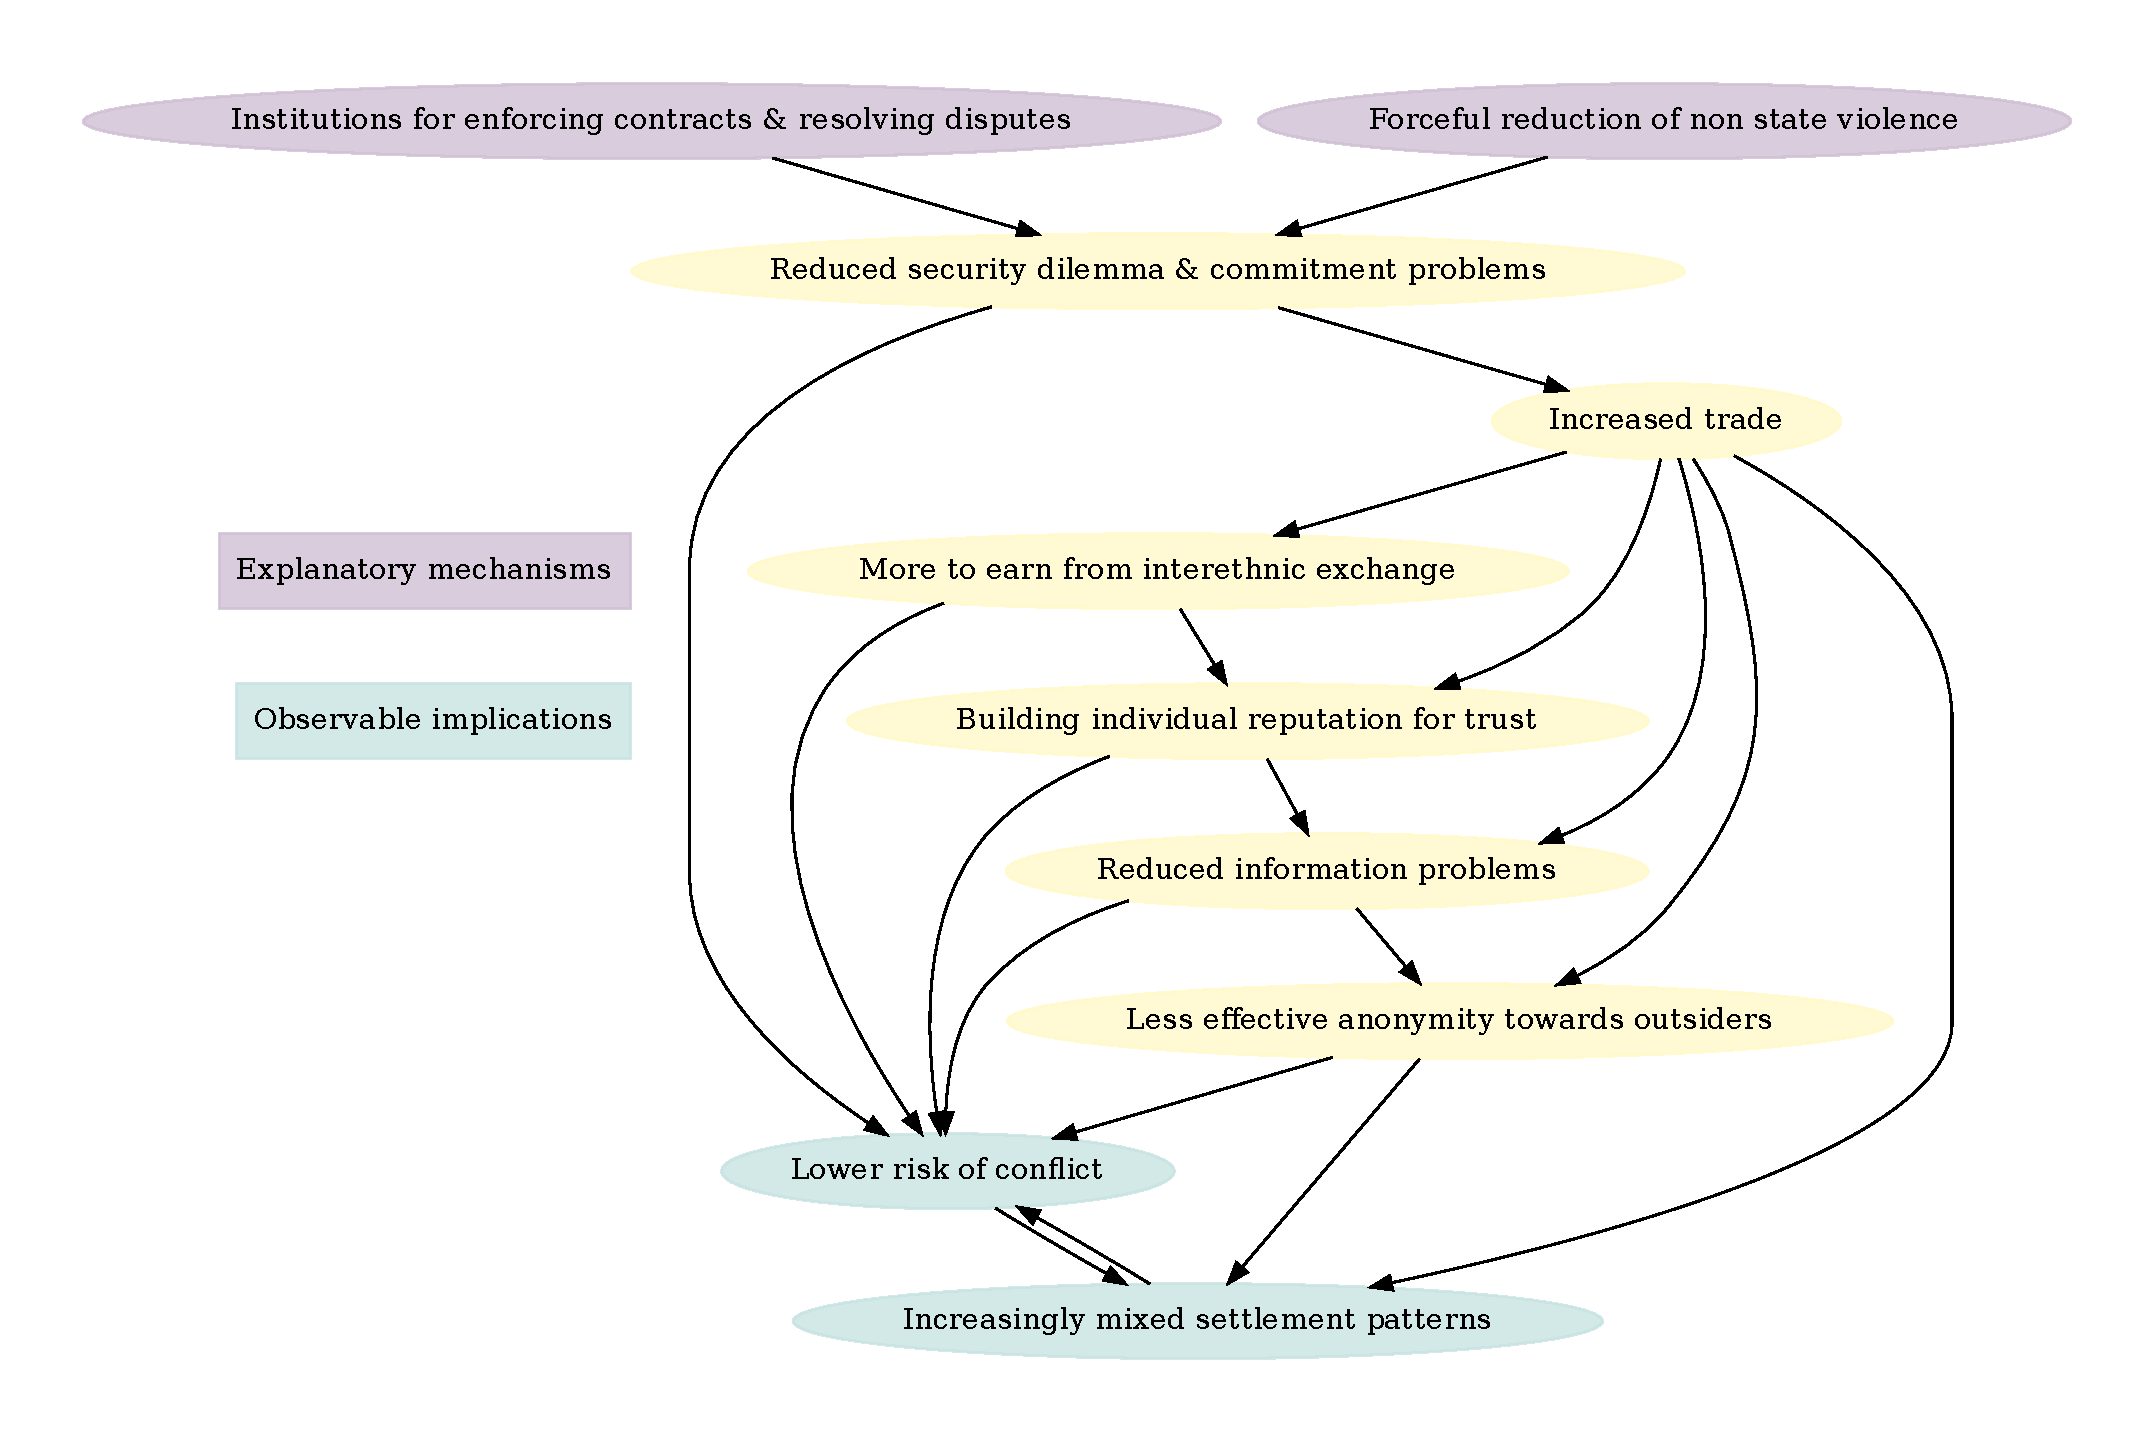
\includegraphics[width=1\linewidth]{img/OMTcausal.pdf}
	\caption{Causal diagram}
	\label{causal}
\end{figure}

In most cases precolonial states were either conquered by other precolonial
states or colonisers (see below). Because the processes that reduce the
information problem over time have been in effect for a relatively longer
period, these areas start at a lower relative level of communal violence in the
postcolonial period. Even in the few cases where previously state controlled
ares have descended into statelessness, improvements to the information problem
could linger. In areas with a history of precolonial statehood there is
therefore a `carryover effect' from its time as an independent state. Given that
the establishment and consolidation of states is what has had the most direct
effect on suppression of raiding and feuding \citep{Pinker2012}, we argue this
is the main avenue through which precolonial states affect postcolonial levels
of communal violence.

\subsection{Precolonial states as building blocks for the postcolonial state}
\label{Precolonial states as building blocks for the postcolonial state}

In order to administer as cheaply as possible, building on whatever
institutional structures that were already in place, became the main policy in
British Africa.\footnote{The principle of indirect rule was written down by Lord
	Frederick Lugard in his (1922) \textit{The Dual Mandate in British
	Tropical Africa.}} The practical difference to other areas, in
	particular French colonies, was minor
	\citep{boone2014property}.\footnote{\citet[31]{englebert2013inside}
		point out that all of French West Africa had 300-400 French
	administrators during the interwar period, necessitating co-optation of
locals and keeping with the cost imperative, implying avoiding a strong break
with the past} Areas with some level of precolonial state presence generally had
existing institutions and at the very least vertical social networks that could
be leveraged by colonizers. This facilitated integrating areas into colonial
administration through systems of indirect rule. Local kings, chiefs and leaders
retained and often had their prerogatives were extended, especially as regards
judicial autonomy, with the colonial power placing itself on top. This
represented an efficient way of cutting administrative costs, despite possibly
undermining precolonial modes of accountability \citep{mamdani1996citizen} for
the colonizers. Thus, when a state existed prior to colonization, colonizers
normally left most matters to the existing rulers -- including courts and the
resolution of disputes, with the exception of a few crucial issues such as
capital punishment (\citealp{boone2014property};
\citealp[30]{englebert2013inside}). If all went as (the Europeans) planned, a
single district commissioner would be sufficient to `guide' the native
authorities. Consequently, European institutions were surprisingly shallow
\citep[25]{englebert2013inside}. Therefore, where precolonial states or their
remnants existed upon colonization, core functions were often incorporated into
the colonial state.

Although received wisdom has it that the precolonial indigenous component to the
colonial states was minor at best, particularly where precolonial states
existed, these often became crucial building blocks in the colonial enterprise.
In the case of Botswana, Lesotho, and Swaziland, colonization was more or less
on request in an effort to fend off Boer conquest. The British willingly
accepted over-lordship of these existing states, largely keeping their
geographical shape and much of their institutional structure. Similarly, Rwanda
and Burundi were colonized in much the shape as their precolonial kingdoms
\citep[45f]{englebert2013inside}. Buganda and Ashanti, in present Uganda and
Ghana respectively, represent two different and illustrative cases of how
colonial conquest of precolonial states were carried out. Buganda is the
prototypical case; after being ravaged by civil war and a crisis of succession,
the Bugandan king accepted German protectorate status in exchange for support
against his rival brother. This protectorate status was then transferred to
Great Britain in exchange for the Heligoland islands in the North Sea only
months later. In Ghana on the other hand, the Ashanti kingdom was eventually
colonized by the British after five Anglo-Ashanti wars, where the British
sustained heavy losses. Despite different initial trajectories. The colonizers
relied heavily on the existing state structures, illustrating that, absent
strong incentives to direct control (strategic resources or areas) European rule
followed a clear cost imperative. 

Even with more direct forms of rule, where local rulers were replaced,
integration was arguably easier than in places with little to no experience of
statehood. Replacing an indigenous hierarchy with another was easier than
building one were none had previously existed. 

In areas where no or little precolonial institutionalization had materialized
societies were quite small -- encompassing often only a few villages -- and
administering them sometimes meant vastly increasing the prerogatives of
leaders, merging smaller groups together into `tribes' by administrative fiat
\citep{boone2014property}. Sometimes, where no real overarching authority
existed, Europeans ended up appointing someone, or inventing historical
precedent out of whole cloth \citep{mamdani1996citizen}. With the obvious
difficulties of administering cheaply by more or less building institutions from
scratch, in particular acephalous societies were much less integrated into
colonial states. Where there was little to build on in terms of precolonial
structures, the colonial state rarely invested heavily in governance unless the
area was of particular economic or strategic value. An area such as South Sudan
where few precolonial state structures existed to build on, was for long
periods of British rule administered by only a handful of colonial
administrators and their soldiers.  

Areas with a more hierarchical political organization were to a lesser extent
partitioned and saw less arbitrary geographic composition than areas without
overarching authorities beyond the immediate villages \citep{Green2012,
Nugent1996}. The brevity of colonial rule also meant that where hierarchical
ruling structures existed before, the colonizers' cost-imperative the
consequence of often leaving a light imprint of statehood. This also meant that
precolonial identities often endured into independence, although often in an
altered (often aggregated) form. 

%Additionally, areas outside the reach of precolonial states were so for a
%reason, usually due to the effective distance (in travel time) from areas able
%to produce a large enough surplus of food to provision armies. The relative
%differences of such conditions had not fundamentally changed despite European
%and more modern armies greater ability to reach such remote areas. Integrating
%remote areas was still relatively more difficult. Being better integrated into
%the colonial administration, and subsequently the nation state, means that the
%conflict reducing mechanisms of state, outlined above, continue to work and even
%at a higher level (of colony and nation state).

%Higher levels of precolonial state presence usually resulted in indirect rule
%during the colonial era. Often this meant more local autonomy in the
%post-independent era, possibly causing such areas to become less integrated into
%modern states than areas of more moderate levels of precolonial state presence,
%and thus enjoy less of the modern states conflict reducing effects. However,
%they do start at a higher level of intercommunal interaction (larger `carryover
%effect'), therefore we argue the overall effect of precolonial state presence
%should remain positive.\footnote{This lack of integration is perhaps evident in
%	the finding that such areas are more frequently engaged in violent
%	conflict with the central government, especially in areas of high
%precolonial state presence far from the capital \citep{Wishman2021}.} 

Upon independence, the new national-level elites hailed mainly from outside
kingly and chiefly families. Fearing the rival power of traditional authorities,
they often tried to weaken traditional authorities at the center in an attempt
to strengthen their own position. At the more local level, decolonization caused
surprisingly little break in substantive terms for the modal country, ending up
with largely reproducing much of the local colonial state structure. Thus,
precolonial entities continued to exert influence into independence, with some
claiming that the indigenous aspects played the main role and that the
colonial state never succeeded in displacing precolonial modes of governance
\citep{ChabalPatrick1999Aw:d}. The mainstream view is closer to what
\citet[22]{englebert2013inside} claim when they say that postcolonial states
have a `mixed parentage' of precolonial and colonial structures.

Africa's independent states did not have to prove their capacity upon
decolonization in order to be recognized internationally as legitimate
entities.\footnote{Keep in mind that unlike a multiethnic \textit{precolonial}
	state like Kanem Bornu, the multiethnic \textit{post-colonial} state of
Kenya never used its \textit{own} instruments/institutions of power to establish
its borders, and incorporate its various ethnic groups.} With an understanding
among African leaders for acknowledging each others' sovereignty, external
threats were a small concern. This exemption of state leaders from creating
effective states \citep{Jackson_1982} has left states often incapable of
carrying out taxation in an efficient manner nor having a monopoly of legitimate
use of violence. Thus, pockets of weak control existed with substantial autonomy
as long as those areas did not rise in rebellion or threaten to secede
\citep[47]{englebert2013inside}. For the same reasons as for the coloniser,
where little hierarchy existed prior to colonization, colonial and postcolonial
states often found it difficult to exert effective control, causing several
developmental liabilities (e.g. \citet{Michalopoulos2013}). For instance,
\citet[8ff]{oba1992ecological} shows that in then Turkana district of Kenya --
which never saw anything close to a state in the precolonial era -- violent
conflicts were quite prevalent before colonization
\citep{muller1989transforming}, with levels of violence during the colonial and
postcolonial period displaying a strong continuity. Despite British intentions
to keep law and order, their inability allowed intergroup clashes producing at
least 800 casualties in the 1929-1958 period as the locals soon realized the
shortcomings of British power \citep[8]{oba1992ecological}. In line with the
argument that with independence much stayed the same at the local level
\citep{englebert2013inside}, raiding persists to this day. 

% 	- the lack of a head chief prevented land rights for certain groups in
% 	Darfur, causing trouble when ecological changes forced these groups to
% 	stay longer on others’ lands (as they had no land on their own)

In sum, the precolonial, colonial, and postcolonial situation in terms of
physical security in an area without precolonial state history has remained
quite `stably unstable'. This means that while the likes of \citet{Pinker2012}
predict an overall conflict reducing trend, and that areas with little/no prior
statehood should see the largest reduction, there is reason to believe that this
his eluded Africa. In other words, that the `carryover effect' has not been made
obsolete by the state building projects of colonisers or independent African
states.

\subsection{Local institutions} \label{Local institutions}

The brevity and light imprint of colonial rule also meant that many precolonial
institutional structures survived colonization \citep{Wig2016, Wig2018},
although often in an altered form. The weakness of current states discussed
above frequently caused them to delegate governance. Particularly for rural
life, power has been devolved to (neo-)customary authorities. Survey data
indicates that the latter enjoy higher levels of legitimacy in crucial aspects,
being seen as playing a more central role than both the local and central
`modern' government \citep[360]{Logan_2013}. Crucially, for many African's daily
life, these authorities are often left with the power to administer land access,
adjudicate disputes, and in general control land in most of rural sub-Saharan
Africa \citep{englebert2013inside, boone2014property, posner2005institutions}.
Traditionally based institutions should generally be more closely tailored to
local conditions than ones created by colonial administration or an often remote
modern state. By being aware of and understanding local traditions, customs, and
culture, such institutions might also prove more effective at resolving
disputes. Precolonial states may for example have left specific mediation
mechanisms such as councils or courts for dealing with potential triggers that
exist between two communities. Additionally, these institutions sometimes tie
agreements to their own good reputation. The breaking of agreements would
jeopardize the institutions themselves. If tied to formal (though not
necessarily state recognized) institutions, contract-breaking would require that
the very same institution overturn its own previous decisions. Such institutions
make inheritor groups more credible partners \citep{Wig2018}. 

% Joking relations an example of this?

The degree to which the traditional authority in question is hierarchically
organized arguably shapes how effectively it can handle conflicts between groups
from spiralling \citep[46]{Wig2018}. One specific institution that was
frequently persisted from precolonial states into the postcolonial period is
leadership. Sometimes they were officially incorporated as part of the state
apparatus (as in the case of Rwanda and Uganda), sometimes recognised as
official ceremonial leaders or at times not recognised by the state at all.
Nevertheless leaders can influence the level of communal violence in at least
two ways. Leaders occupy a unique role that allow them to act as mediators -- both
preventing conflicts from escalating to violence and helping bring an end
violence. Even ceremonial leaders have acted as key mediators in not only local
but even national level conflicts (with their higher escalatory potential) as in
the case of Baongo the second, the Mogho Naba -- monarch -- of the Mossi kingdom
in Burkina Faso, who played a key role in brokering the return of civilian rule
to Burkina Faso following a military coup in 2015
(\href{https://www.bbc.com/news/world-africa-34340704}{BBC}). Leaders whose role
hails from precolonial hierarchical structures such as states are uniquely
placed also to make more credible commitments as they are better placed to
prevent and punish potential spoilers \citep{Wig2016}.

% \subsection{Economic development?} \label{Economic development?}
% 
% Better integration with colonial administration and national state could give
% precolonial state ares a competitive edge relative to other areas when it comes
% to developmental projects and priority from the government. If so that should be
% reflected in higher levels of economic development, which is famously linked to
% lower levels of conflict. However, this relationship could have been turned on
% its head by the "reversal of fortunes" \citep{Acemoglu_2002}. Additionally,
% finding accurate measures of subnational (or even national) economic development
% is a while can of worms.

%With the central role land plays in the daily life in
%rural Africa, this gives traditional authorities considerable power at the local
%level. 
%
%- use Wig \& Kromrey (2018,p 5: first para) on another study
%finding that land allocation often delegated to groups with formal customary
%institutions - that is precolonial states or state-like structures. (Boone uses
%a similar argument, as does Posner on Zambia).
%- something on mechanisms
%    - in group mediation
%    - outside commitments
%    - intergroup interaction
%    - within group interaction
%
%    - see Wig \& Kromrey (2018:2) on how customary institions, including precolonial states, have been integrated in colonial and postcolonial states .
%        - Wig \& Kromrey (2018:5) use the Zulu kingdom and other case as examples where precolonial institutions (not sure if all are classified as states - Marius?) handle disputes: OMT check these!
%		- RESPONSE (MSW): Zulu is definitely in there, but not a very `thick' presence.
%		What are the others?
%
%
%    - see Beyene (2009) - no does not work - conflict resolution, but no precolonial state
%
%
%        - TAB ON MALI?
%
%
%        - HAGBERG ON BURKINA FASO?
%        
%        
%        - How these institutions are still in place and help keep the peace [ideally, if possible, can these institutions be shown to resolve any of the dilemmas addressed above?]
%        
%        - THESE CASES CAN BE USED TO COUNTER THE ARGUMENT ON THAT PASTORALISM IS PROBLEMATIC
%        
%        
%        Turner et al. (2012:749f) on that in resolving disputes, people prefer turning to traditional/customary authorities before national
%        
%        
%      
%        - Breusers et al. (1998:375ff) "Mossi farmers and Fulbe herdsmen have lived together for a long time on the Central Plateau of Burkina Faso" : 
%            - Marius how is the precolonial state presence here? (this is the Mossi Plateau where the Mossi kingdom has existed since the 12th century)
%	    	- RESPONSE: See figure \ref{brkplots} in appendix. Values are
%		normalized on the sample shown (not global sample)
%            
%            
%                - there were precolonial states that incorporated both: not present any more, but long-standing intereth relations
%        
%    - add that the national level elite and their lack of concern for local
%	dynamics is of secondary importance to our argument, but of some
%	relevance for understanding communal violence [Elfversson 2015; ++].
%	Thus, the internationally guaranteed sovereignty reduces the impetus to
%	rule effectively domestically. The postcolonial states is 'able to
%	largely reproduce the colonial blueprint and rule with limited
%	constraint and accountability, practicing their authority as command'
%	(Englebert \& Dunn 2013:52). Hence, unless crucial, many areas are left to fend for themselves. In the case of precolonial state structures/institutions still being somewhat operative, these sometimes do fill the void.
%    
%- South Sudan was governed indirectly without much precolonial states]
%
%- argument about legal pluralism (Englebert \& Dunn 2013:30f; Eck 2014 on communal violence and legal pluralism)
%

\section{Observable implications} \label{Observable implications}

\subsection{Communal violence} \label{Communal violence}

While we expect that precolonial states generally decrease post cold war levels
of communal violence, we do not expect this effect to be uniform across the
former territory of that state. Just as today's states are unable to uniformly
control their territory, the precolonial states of Africa had zones with varying
degrees of control and influence (broadly conforming to concentric circles
extending form the capital). Thus, we expect any pacifying effect of precolonial
states to vary according to the local degree of that state's presence.

\bigskip
\hangindent = 3.5em \textit{H\textsubscript{1}: Higher levels of precolonial
	state presence decrease local levels of communal violence.}
	% Or should we express it in terms of low levels of state presence ->
	% more violence?
\bigskip

It is important to note that, because our theory only speaks to horizontal intra
group conflicts (communal violence), we do not expect this relationship to hold
for other (vertical, primarily state-based) types of conflict. 

\subsection{Mixed settlement} \label{Mixed settlement}

Non-state conflict resolution mechanisms such as IGP, require that in-groups are
sufficiently homogeneous or tight knit to be able to locate and punish
perpetrators. In other words, where groups are, or have been, self reliant in
terms of intergroup conflict resolution, we expect high levels of ethnic
homogeneity. Additionally, the causal relationship we suggest implies that there
is a positive feedback loop running between less communal violence and more
mixed settlement. As the state reduces the security dilemma and commitment
problems, inter group economic and social interactions increase (see Figure
\ref{causal}). In particular this leads to less effective anonymity towards
outsiders, which makes hiding amongst coethnics less effective. Furthermore, the
lower risk of conflict, means that economic opportunities and other concerns can
take precedence over security, when making decisions about where to live. Given
that this relationship likely works both ways -- outbreaks of ethnic violence
(communal or state based) drives homogenization among previously mixed
settlement groups -- it is difficult to determine the causal direction.
Nevertheless we expect to see more mixed settlement patterns in areas with more
precolonial state presence, than in areas with less precolonial state presence.

\bigskip
\hangindent = 3.5em \textit{H\textsubscript{2}: Higher levels of precolonial
	state presence allows for more ethnically fractionalized settlement
patterns at the local level.}
\bigskip

%On the face of it, it might seem counter intuitive to expect less communal
%violence in areas with more mixed settlement, and there is some truth to this
%intuition. In a setting of mixed settlement there are a lot more potential
%triggers to conflict as people are interacting more frequently, simply as a
%consequence of proximity. This is precisely why, absent effective conflict
%prevention, communities tend to cluster along ethnic (or other identity group
%lines).

% \subsection{Interethnic trust} \label{Interethnic trust}
% 
% The hypothesised increased interethnic interaction and longer periods of
% stability between ethnic groups within precolonial state areas should over time
% lead to a relative increase in trust toward other groups. While the increased
% interaction only happens among the groups within the precolonial state territory
% and neighboring communities, these groups are also likely to be the reference
% point for people when asked about trust in non-coethnics.

%\subsection{Norms of hospitality and conformism in nonstate societies?} \label{Norms of hospitality and conformism in nonstate societies?}

% Is this observable?
% Does this belong under how non-state groups handle stuff?

% This creates cultures that encourage nosiness in coethnics affairs, and norms of
% thick-skinedness, extreme self-restraint, generosity, hospitality and politeness
% towards outsiders\footnote{Thus the first section of the main text Hávámal on
% 	Norse norms, literally ‘the guest’s section’ (Gestaþáttr) of Hávamál
% 	contains maxims allegedly given by the head deity Odin to men for proper
% 	conduct in a nonstate society inducing almost sacred norms of
% hospitality and reciprocity towards stranger guests, but also patience and
% cautiousness on behalf of the visitor.}, and strongly discourage hot-headedness.
% In the words of \citet[37]{Colson1974} cited in \citep[199]{Cohen2004} ‘people
% live in what appears to be a Rousseauian paradise because they take a Hobbesian
% view of their situation…’ going out of their way to avoid those single acts of
% aggression they fear will cause long spirals of violence. However, as the strong
% emphasis on norms of ‘niceness’ towards outsiders in peacetime reflects, these
% societies are found to be much less effective at containing violence once
% cross-ethnic disputes occur as the failure to retaliate violently would reduce
% the credibility of this deterrent strategy \citep[723f]{Fearon_1996}.

% Pinker og høfflighet i sørstatene kontra øst-kysten, kan vi knytte det til
% frykten for at det skal eskalere til gruppe konflikt


% \subsection{Stronger effect of PCS presence in British colonies?} \label{Stronger effect of PCS presence in British colonies?}
% 
% If the assumption that the British to a larger degree ruled their colonies
% through indirect rule than other colonisers, then according to our hypothesised
% ease of integration and local institutions mechanisms should work better in such
% areas. However, this difference in colonial strategy is often exaggerated and
% stems more from different official aims than form any real difference in de
% facto policy on the ground.

\section{Research design} \label{Research design}
\subsection{Main analysis} \label{Main analysis}
 
Our explanatory variable is time invariant. This means that we are limited to
doing a cross sectional analysis. If we were to attempt to panel data analysis
we would essentially be repeating the same experiment multiple times with
observations that are wrongly assumed to be independent of each other. 
% Opportunity to take down other recent papers who "solve" this by interacting
% their variable with something that varies (only slightly) over time.
Because our inquiry is spatial in nature we use .5\degree \hspace{1pt} by
.5\degree \hspace{1pt} grid cells, using the PRIO-grid system and cell-id's
\citep{Tollefsen2012}. Using such a grid cell approach has the benefit of
avoiding any potential bias introduced by using, for example, administrative
units that might be derived from precolonial borders.

Similarly, the treatment far precedes measurement which creates the potential for
posttreatment bias. This means that in selecting control variables we have to
weigh the potential for introducing posttreatment bias against potential omitted
variable bias. Accordingly we add control variables stepwise with increasing
likelihood of introducing post treatment bias.

Because our dependent variable for H\textsubscript{1} is a count variable
(number of communal violence events), we use a negative binomial regression
model.\footnote{A likelihood ratio test confirmed that a negative binomial model
was a better fit than Poisson.} The dependent variable also contains excess
zeros, and because we cannot know for certain the data generating process behind
all zeros we include zero inflated negative binomial (ZINB) as well. We used the
same set of independent variables for the first and second step of the ZINB
models as we do not expect any of the variables to only affect onsets (first
event in a given cell) and not conflict severity (number of events in a cell
that has at least one event), or vice versa.

As is clear from Figure \ref{logOrg3}, communal violence in Africa primarily
occurs in two large clusters. In East Africa most events are in Kenya and
Uganda, and in West Africa most events are in Nigeria and a smaller cluster in
Ghana. We therefore ran several split sample regressions (see Figures \ref{zorg3},
\ref{znon_state} and \ref{zacledev}).

% Spatial lag models?

For H\textsubscript{2} we employ a regular OLS-regressions. 

\subsubsection{Dependent variables} \label{Dependent variable}

For the main analysis our dependent variable is communal violence events per
grid cell in the 1989-2020 period, as captured by the `Organizational level 3'
variable from the UCDP Georeferenced Event Dataset (GED) and corresponding UCDP
Non-state conflict dataset. This corresponds to events in which conflicts
between `informally organized groups' surpass a yearly threshold of 25
battle-related deaths in a year, and is meant to capture `communal conflicts'.
In the appendix, we also include models using all non-state state conflict
events, as well as equivalent communal violence events in the Armed Conflict
Location and Event Data (ACLED) \citep{Raleigh_2010}.

\subsubsection{Independent variable} \label{Independent variable}

The main explanatory variable is precolonial state presence, as measured by the
main aggregated variable of the Georeferenced International Systems Data
(Geo-ISD) \citep{Wishman2021}. Based on hundreds of maps from the period
1800-1914, complimented by historical atlases compiled by later historians, it
measures state presence by counting how many maps place any given state from
the ISDv2 within each PRIO-grid cell per year. By layering the shapes of each
state (as drawn in the maps) the Geo-ISD is able to leverage the variation in
the different sources' conceptualisation of statehood, as well as variations
over time, to create a three dimensional measure of historical state
presence.\footnote{As opposed to the traditional two dimensional, Cartesian,
representation of most international maps.} Most sources draw borders
encompassing the core areas of a state. Outside core areas, fewer maps overlap,
and further away still, even fewer maps overlap. This creates a measure with
fuzzy borders which approximates the theory of state presence as a series of
concentric circles. Such a fuzzy measure is particularly suited for precolonial
Africa, where very few states had anything resembling well stipulated
international boundaries.\footnote{Exceptions include the border between Borno
and Sokoto for parts of the period, and Western settler states.} Indirect and
nominal rule, far from a European import to the continent, was widespread, and
any traces left by such states would vary with the degree to which the state
actually controlled that area. The definition of `state' that is used is derived
from the ISDv2 \citep{Butcher2020}. The ISD records sovereign states across the
1814-2016 period, defined as a political entity with a population of at least
10,000, autonomy over a specific territory and sovereignty that is either
uncontested or acknowledged by relevant international actors
\citep{Butcher2020}.\footnote{For a more in depth discussion of the definition
of and criteria for statehood that the ISD is based on, see
\citet{Butcher2017}.} We use the measure of state presence that includes
interpolated years from historical atlases (shapes are drawn across all years in
which historical atlases depicted borders over a range of years). For a further
discussion of the precolonial state presence measure see \citet{Wishman2021}. 

\subsubsection{Controls} \label{Controls}

In the first, baseline model, we control for various potentially confounding
geographic characteristics that could affect both state creation and communal
violence. 

We control for how mountainous a grid cell is on average because this could
influence state building, by making it more difficult for people to leave the
oppression of a state \citep{Carneiro1988, scott2017against}, and by providing
natural defences. At the same time mountains affect population density
negatively which affects both state building and conflict events. Generally
speaking fighting occurs where there are at least some people. Lastly,
mountainous terrain can be more difficult for a modern state to reach, and so
the same mechanisms we describe for the state ability to repress communal
violence might work independent of precolonial state presence. The variable is
sourced from the PRIO-grid data set \citep{Tollefsen2012}, but originally from
\citet{Blyth2002}, and measures the percentage of the cell with mountainous
terrain based on elevation, slope and local elevation range.

% Could actually be a matter of catching pockets of low state presence within
% otherwise "stated" territory.

Similarly, access to water is a key ingredient of state building, while it also
proxies population density to some degree (people tend to live near water).
Additionally, communal conflicts could erupt over access to water, either
drinking water, for people or herds, or for irrigation \citep{Doring2020, Detges_2014}.
We use a measure of water as a percentage of the grid surface, which is included
in the PRIO-grid data set, but originally from the European Space Agency
\citep{Bontemps2009}.

We also included a measure of how much of a cell is barren, as a proxy for
population density. People generally do not live in barren areas, and so we do
not expect a lot of fighting there. At the same time we do not expect states to
proliferate in barren areas. The data is from \citet{Bontemps2009}.

The mean distance to the coast of each cell could be positively correlated with
state building through the coastal slave raiding and trading states of the
period, as well as to economic development \citep{Nunn2008}. Because economic
development is expected to reduce the risk of conflict, distance to the coast
could represent a confounding variable. We use data from \citet{Wessel1996}, and
the variable is log transformed to account for a non-linear relationship.

Lastly for our baseline model we include a proxy for land not suitable for
pastoral herding. The variable is coded as 1 if a cell receives on average more
than 400mm precipitation per year, and otherwise 0. We include this variable
because a typical set of cases of communal violence are events related to cattle
raiding and conflicts between pastoral herders and settled farmers. Thus, if
these dryer areas are also more or less suitable for state building this would
represent a confounding variable. The precipitation data used to construct this
variable is from \citet{Schneider2015}.

In the second model we control for North Africa because of how overrepresented
North Africa and Morocco in particular is in the state presence data. If North
Africa also has experienced more or less communal violence than the rest of
Africa, it would bias the estimated effects.

In the third model we control for population density in 1600. As already
mentioned, population density (log) predicts statehood because states need a
certain level of population density in order to form. At the same time violence
only happens where there are people. The data was sourced from the HYDE project
\citep{Goldewijk2016}. We choose the year 1600 because it should be far enough
back in time to be before the establishment of most of, although not all, of the
precolonial states in the data, and thus also avoid post treatment bias. This
measure is however partly based on interpolation back in time, and so is
excluded from the baseline model out of caution. 

\subsection{Ethnic fractionalization} \label{Observable settlement patterns}

For H\textsubscript{2} we construct an ethnic fractionalization index using the
universal application of the Herfindahl–Hirschman index.\footnote{\(EF_c = 1 -
	\sum_{i=1}^nS_i^2\), where \(EF_c\) is the level of ethnic
	fractionalization in grid cell $c$, $i$ indexes ethnic groups, and
	\(S_i\) is the proportion of the population in unit $c$ belonging to
ethnic group $i$ (\(i = 1, …, n\)).} Higher scores on the index indicate more
ethnically mixed settlement. To construct this index, we aggregate high
resolution interpolated data on ethnic group settlement patterns from the SIDE
project \citep{M_ller_Crepon_2018}, to the PRIO grid cell level. Unfortunately,
the data is not available for all of Africa, only for a selection of countries
and years, i.e. a non-random sample. Cells with negative values due to overlap
between two countries included in the SIDE data were excluded, as were scores of
>= 1. The resulting index for the available countries can be seen in Figure
\ref{ethplot}. The reason for aggregating the data is to be better able to
control for potential confounding variables. Without controlling for population
density, sparsely populated areas can get extreme values that bias coefficients.
An example of this can be seen in Figure \ref{ugaplots}, where there appears to
be very high levels of ethnic fractionalization in the middle of Lake Victoria
(bottom right of the left plot), where maps have consistently drawn the borders
of the Buganda kingdom along the coast of the lake, resulting in low scores of
precolonial state presence (bottom right of the right plot). Given the potential
for post treatment bias in the population density measure, we first do a
baseline model controlling for percentage of surface covered by water and
percentage of cell that is barren. In the second model we control for population
density as well. These controls as well as the independent variable measuring
precolonial state presence use the same data used in the main models.

Because of the aggregation, and the non-random and limited sample, we also
include plots of ethnic fractionalization in the full resolution of the SIDE
data for the four countries with communal violence. The more detailed plots
allow for side-by-side visual comparison of ethnic fractionalization to equal
resolution data on pre-colonial state presence.

\section{Results} \label{Results}

Our main models find the expected negative relationship between state presence
and communal violence that is consistently significant, but only after
controlling for population density (see Table \ref{org3} and Table \ref{zorg3}
for main results). This is not surprising however, given the importance of
population density in both state creation and communal violence. In other words,
the baseline and North Africa models are both suffering from omitted variable
bias. In terms of controls, the variables behave more or less as expected.
Mountainous terrain is consistently positive and significant across all models.
Water is positive, but only significant after adding population density, and is
not significant in the ZINB model. Barren terrain remains close to zero, and
changes sign after adding population density, but is positive and significant in
the ZINB models. Distance to coast is positive and significant across the
negative binomial models as well as in the second step ZINB model. Land not
suitable for pastoral herding is not significant in any of the negative binomial
models, but is negative and significant in the communal violence count models.
In line with the theoretical expectation of spirals of reciprocal violence, this
suggests that when communal violence breaks out in areas suitable for pastoral
herding, events tend to repeat. As expected, population density is positive and
significant across all model specifications. 

The results of the zero-model (first step of the ZINB) are perhaps a bit
surprising, and counter to our theory, as precolonial state presence is not
significant (even while controlling for Nigeria, see discussion about regional
variation below). In other words, precolonial state presence does not
significantly predict whether a cell has an initial outburst of communal
violence, but if it does, precolonial state presence significantly reduces the
number of further events. This implies that institutions left by precolonial
states and/or the carryover effect from past pacification works best to
deescalate conflict once it erupts, rather than preventing conflict from
occurring in the first place. However, it could be due to a combination of how
the data is coded and regional variations, as when controlling for the effect of
Nigeria the term (precolonial state presence on likelihood of zero), is
significantly positive. As our theory suggests.

In terms of substantial effects Figure \ref{mainmodels} reports the predictions
of our main models. The main models reveal a modest, but significant effect. As
explained in section \ref{Main analysis}, the ZINB model shows the predicted
\textit{additional} communal violence events in cells with at least one event.
Thus it is more so a measure of communal violence severity. Based on the main
ZINB model, going from zero to an average amount of precolonial state presence
is enough to reduce the number of predicted additional events by one.\footnote{
This prediction is for lands suited to pastoral herding, outside North Africa,
and all other variables held constant at their mean. For non-pastoral lands the
equivalent is a 0.7 reduction.}

\begin{figure}[htpb]
	\centering
	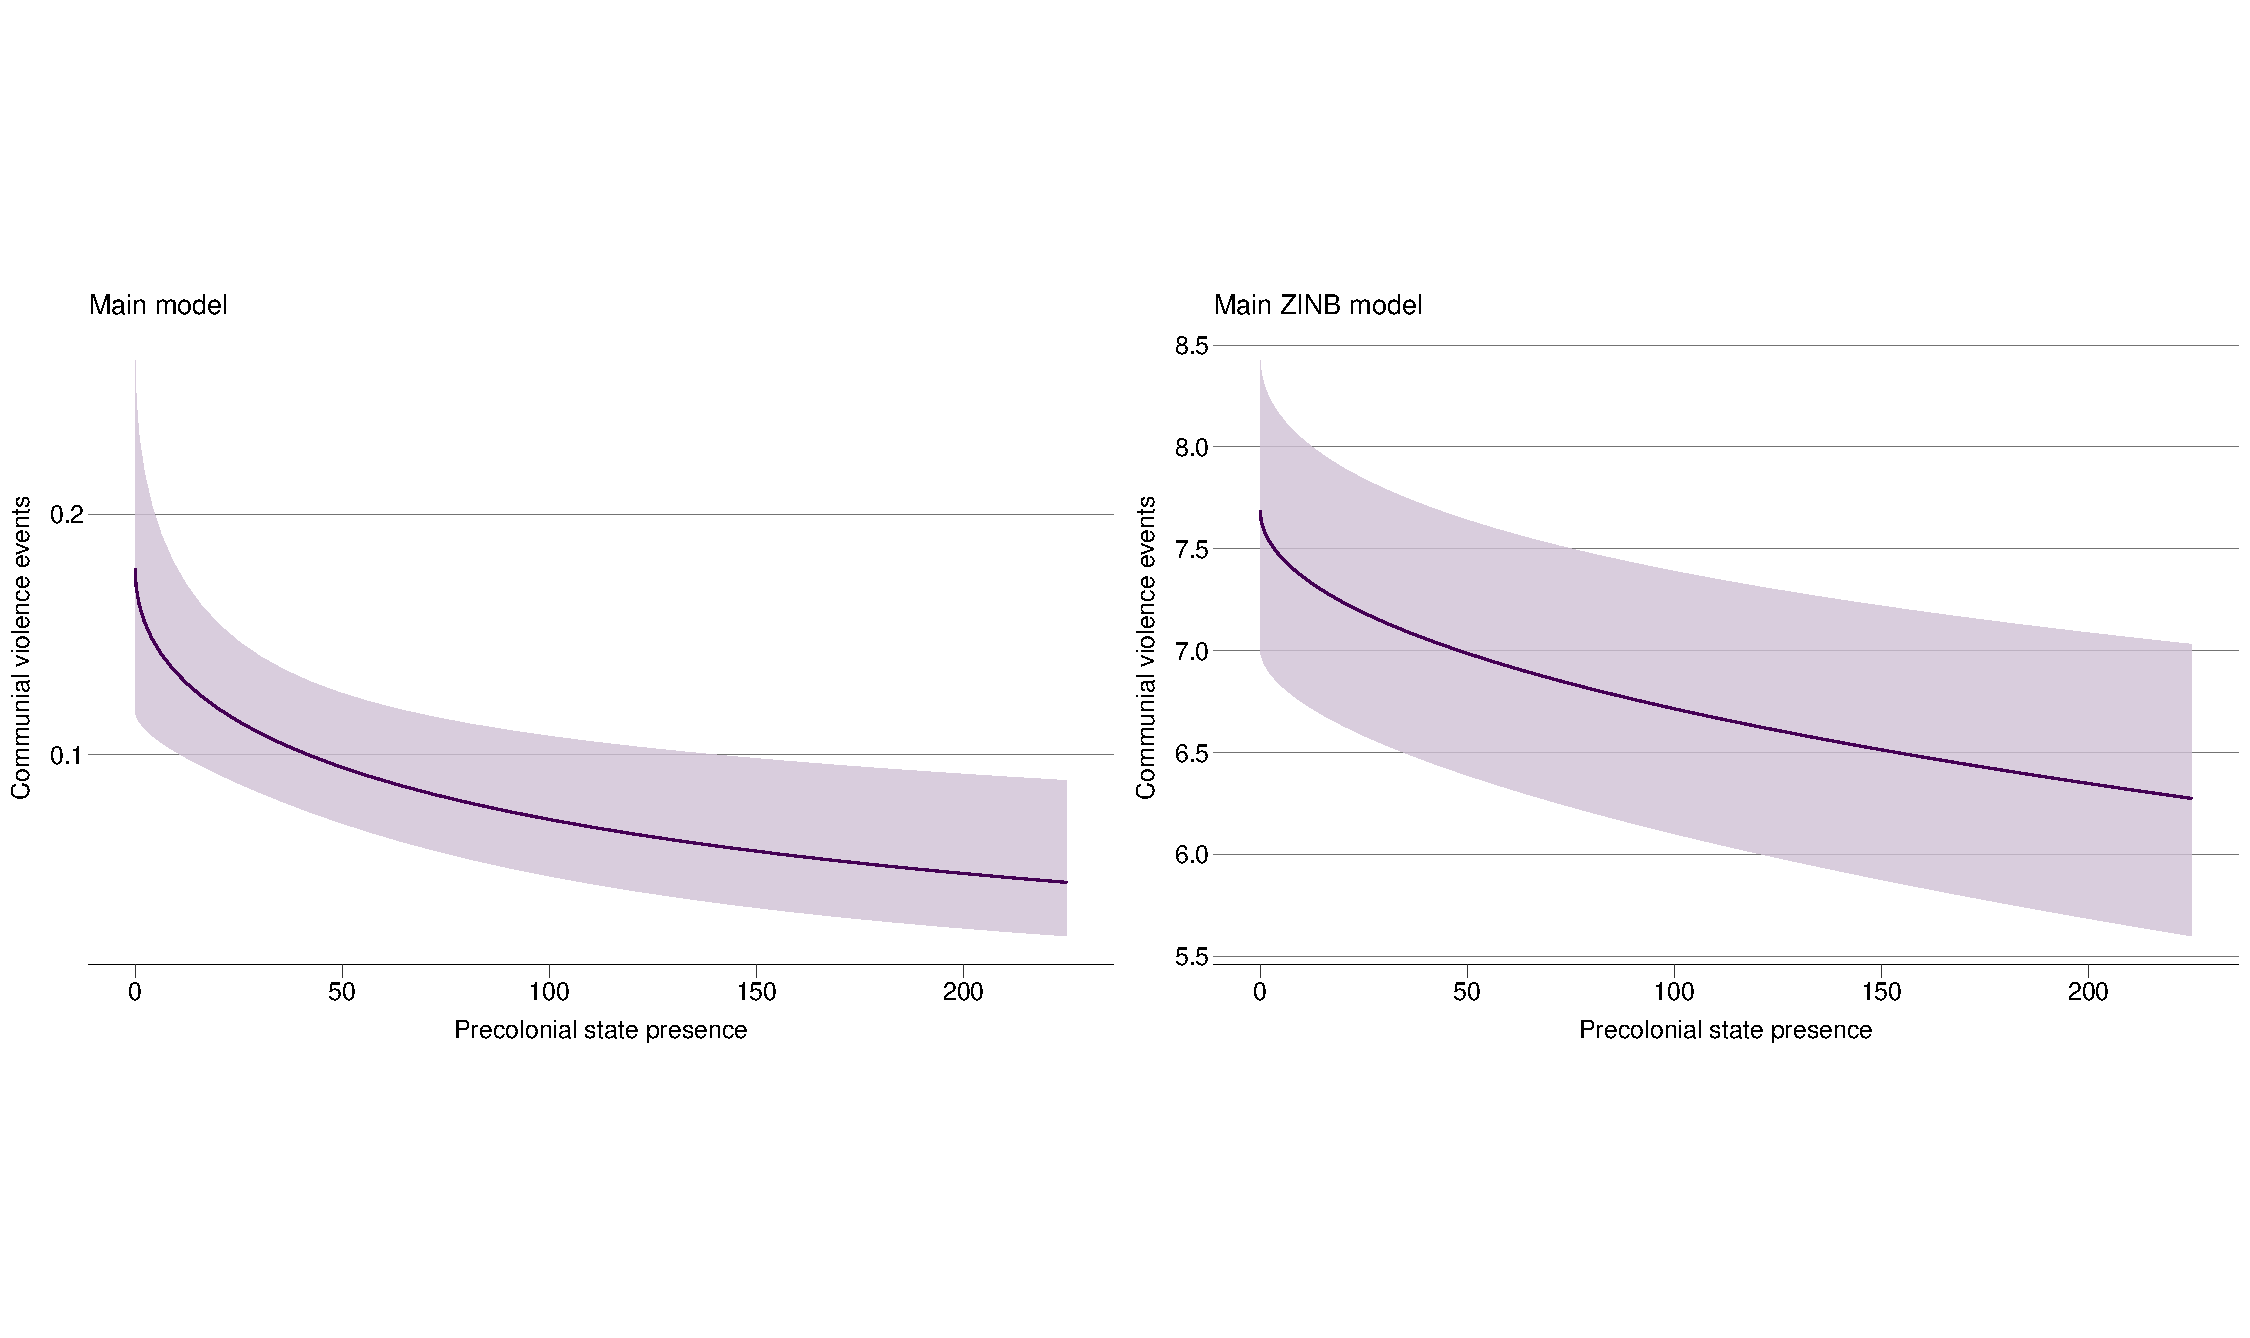
\includegraphics[width=1\linewidth]{R/Output/mainplots.pdf}
	\caption{Main model predictions}
	\label{mainmodels}
\end{figure}

Overall the results indicate a modest, but significant effect of precolonial
state presence on communal violence, that is in line with our theoretical
expectations. However, looking at the spatial distribution of the dependent
variable, as shown in Figure \ref{logOrg3},\footnote{Log-transformed to
facilitate visual interpretation of the data, given its skewed distribution.}
it is evident that there are large regional variations in communal violence
events. We therefore conducted additional regional analysis.

\begin{figure}[htpb]
	\centering
	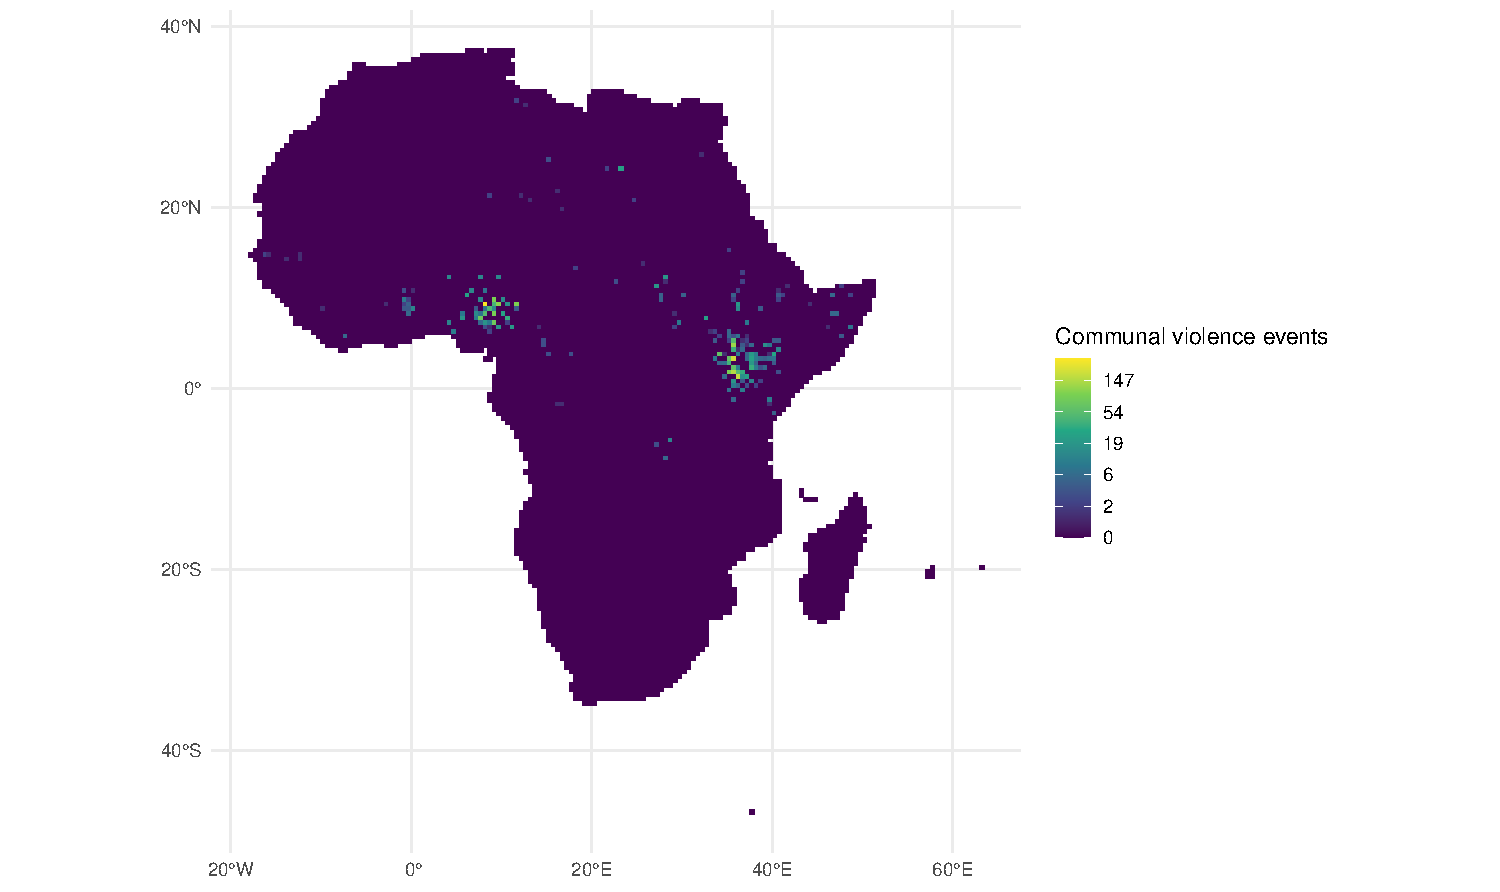
\includegraphics[width=1\linewidth]{R/Output/logOrg3.pdf}
	\caption{Communal violence events (log)}%
	\label{logOrg3}
\end{figure}

\subsection{Regional variation} \label{We need to talk about Nigeria}

The split sample regressions revealed that some other process is probably driving
the results in Nigeria than in the rest of the sample. While the results from
the whole sample do support a general effect in line with our theory, this
effect becomes stronger and more in line with our theoretical expectations if we
exclude Nigeria from the sample, as shown in Figure \ref{znigeria}.

\begin{figure}[htpb]
	\centering
	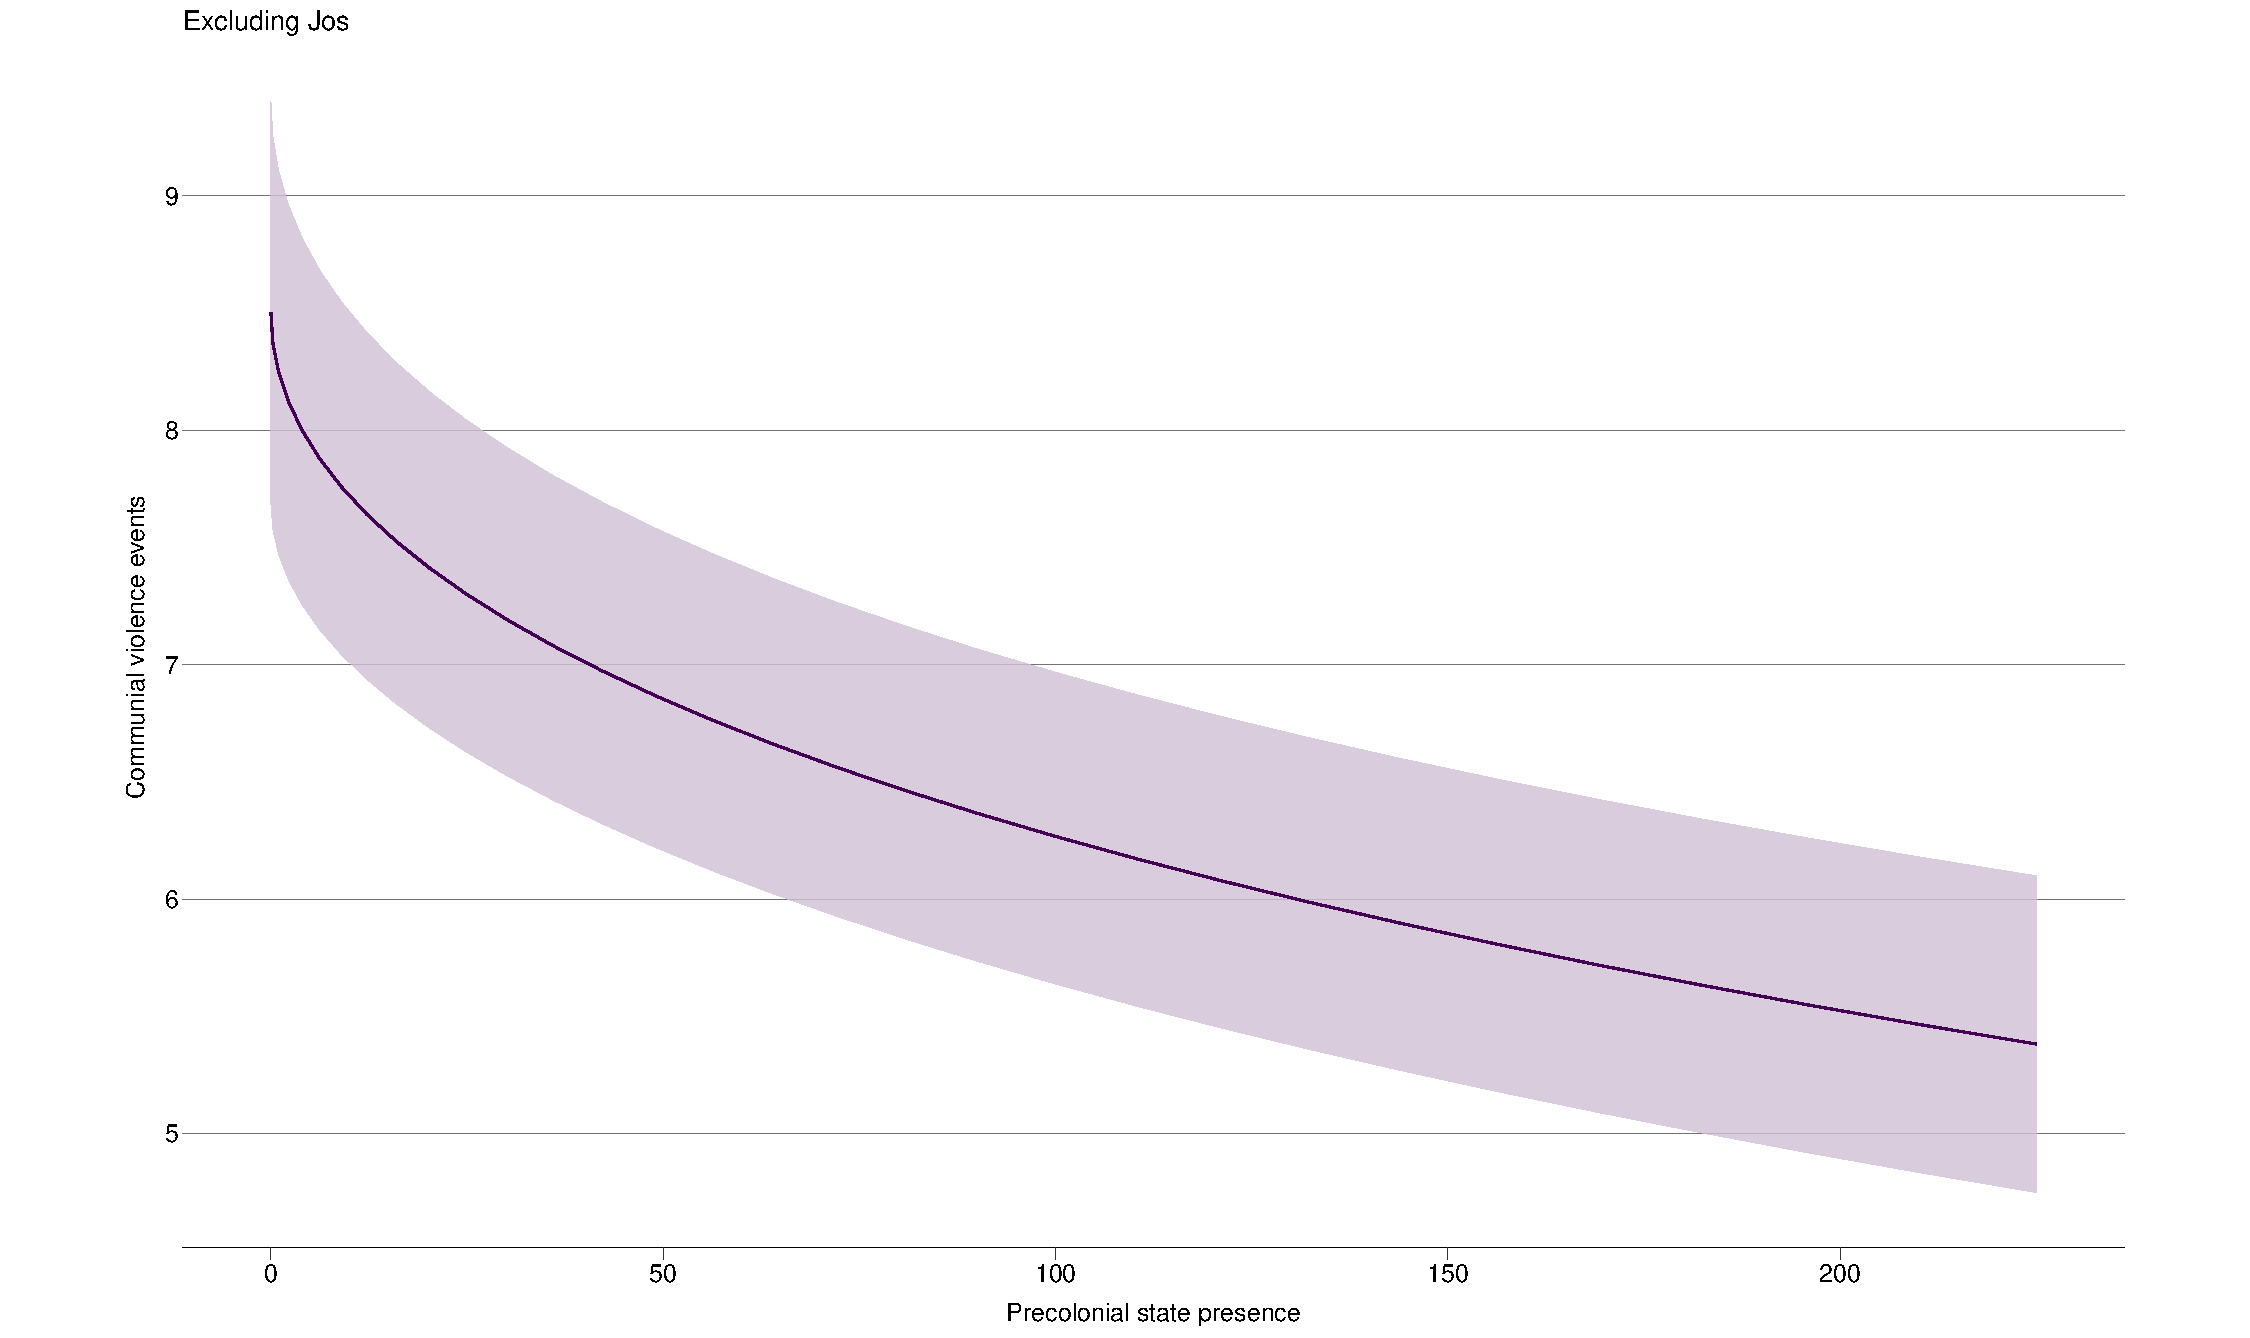
\includegraphics[width=1\linewidth]{R/Output/znigeria.pdf}
	\caption{ZINB count model excluding Nigeria}%
	\label{znigeria}
\end{figure}

It is difficult to determine exactly what is driving the results in Nigeria
without an in depth case study (which is beyond the scope of this article).
However, we suspect it is because most of the cases can be tied to national
cleavages and politics. In Nigeria the fault line between the Christian
dominated South and the Muslim dominated north, not incidentally, runs along the
borders of the Northern precolonial states of Sokoto, Adamawa (at times part of
the former) and Borno. A great deal of the communal violence in Nigeria happens
between the two religious communities, meaning that events in one location can
trigger new events elsewhere in the country. This is highlighted by the UCDP
description of the Muslim-Christian conflict dyad in Nigeria. The localization
of the fault line also means that most of this violence happens in the high
precolonial state presence areas of the aforementioned states. Figure
\ref{noreligion} shows that despite removing the events coded in the GED as
belonging to this dyad, the results are largely the same. However, as the UCDP
notes in the Muslim/Christian dyad description it is very difficult to decide
whether or not events belong to this dyad, as most events follow the fault line,
but differ in which Muslim/Christian groups were involved and what other factors
were relevant. In the end the GED only coded events with overtly religious
motivations as belonging to the Muslim/Christian dyad. Thus the national
divisions are likely influencing the remaining events as well. This is very
different from the local disputes and security dilemmas that our theory
describes. 

An alternative explanation of the diverging results in Nigeria is that the
mechanisms we propose in section \ref{What lingering effects do precolonial
states have today?} only apply to East Africa. Figures \ref{org3plots} and
\ref{non-stateplots} include interaction models for East and West Africa to
show how the effect of state presence differs across the regions. However, these
results are largely driven by Nigeria. Therefore, we also include an interaction
model demonstrating the effect of state presence in Ghana. In all the models
using the GED events data (Figures \ref{org3plots}, \ref{non-stateplots} and
\ref{noreligion}) state presence has a positive effect in Ghana as well. This
suggests that state presence does indeed affect communal violence differently in
West Africa, and that our theory only seems to apply well to East Africa.
However, the model using the ACLED communal violence events provide contrary
results. As shown in Figure \ref{acledplots}, state presence has the predicted
negative effect on ACLED communal violence events in Ghana. Additionally, the
positive effect in Nigeria is far less pronounced. In conclusion then, the
results for West Africa are inconclusive and sensitive to the measurement of the
dependent variable. Nevertheless, the general effect is robust across all models
and measurement choices.

\subsection{Settlement patterns} \label{Settlement patterns}

Table \ref{sidetable} shows the results of the analysis of ethnic settlement
patterns. Precolonial state presence has a positive and significant effect on
ethnic fractionalization, albeit substantially modest. Control variables are of
less concern, as we do not have clear expectations for effect (because low
population density could lead to extreme values in either direction). While this
general finding is consistent with our expectations, the more detailed plots are
arguably more interesting, and merit further discussion.

% TODO: Fix name of legend, and the lack of an upper border.
\begin{figure}[htpb]
	\centering
	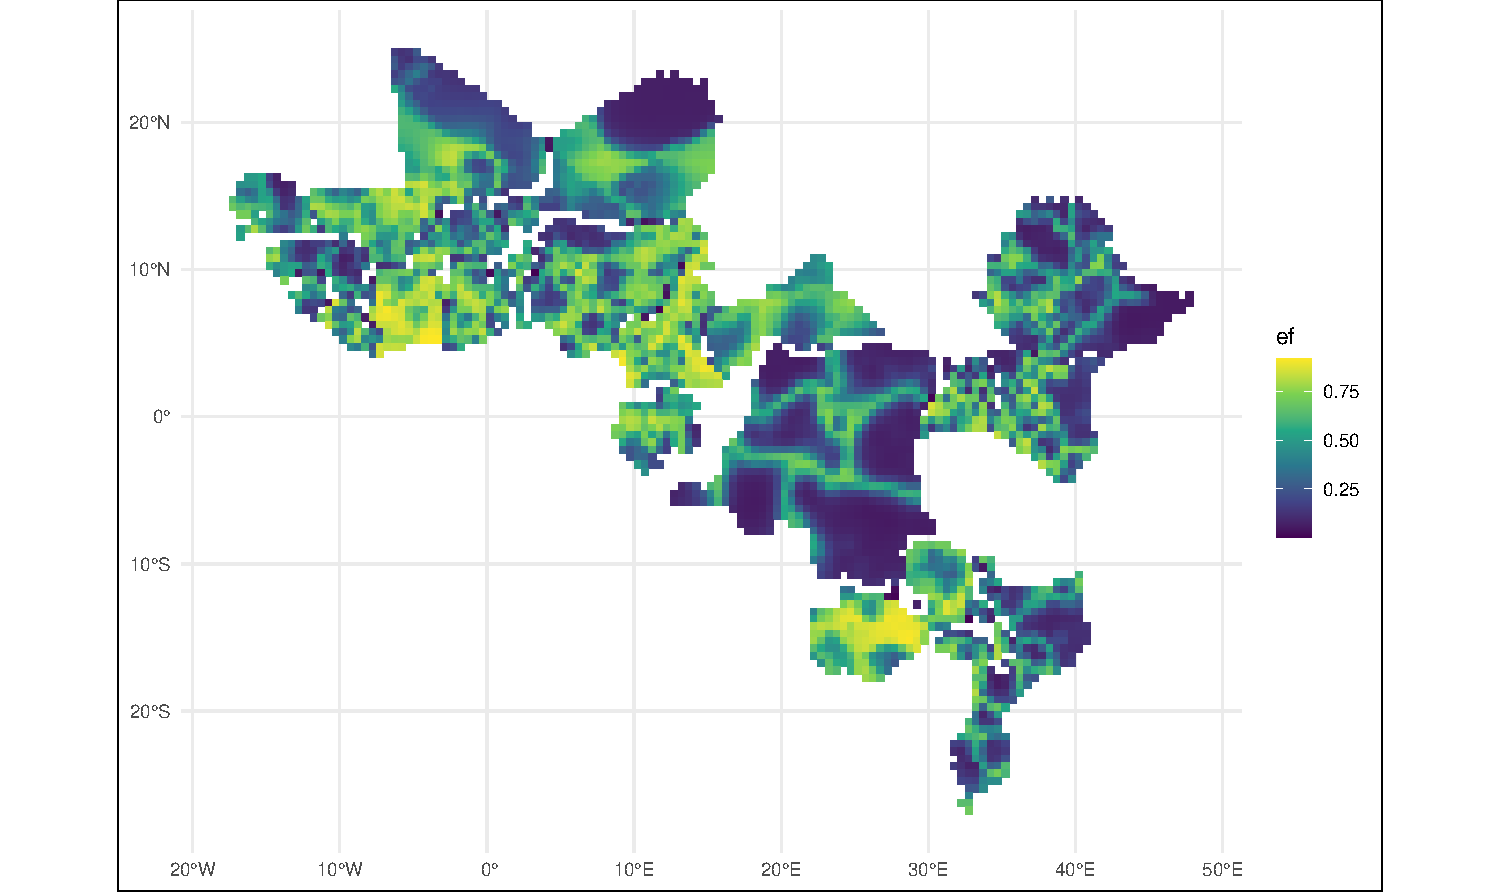
\includegraphics[width=1\linewidth]{R/Output/ethplot.pdf}
	\caption{Ethnic fractionalization}%
	\label{ethplot}
\end{figure}

Figures \ref{ugaplots} to \ref{kenplots} show side by side comparisons of ethnic
fractionalization and state presence in Uganda, Nigeria, Ghana and Kenya. The
settlement patterns in Uganda  (as seen in Figure \ref{ugaplots}) are the ones
that most clearly conform to our theoretical expectations. In the relatively
(precolonial) stateless North of the country, groups live in homogeneous bubbles
separated by corridors of high ethnic fractionalization. These corridors are
presumably low population areas, or `no-go zones'. The result is a
cell-like\footnote{As in biological cell, not grid cell.} settlement pattern.
This does not appear to be an exclusively Northern Ugandan phenomenon, as the
other clearly visible zone of ethnic homogeneity is in the low state presence
south West corner, which was an area largely outside the control of the Buganda
and Bunyoro kingdoms.

\begin{figure}[htpb]
	\centering
	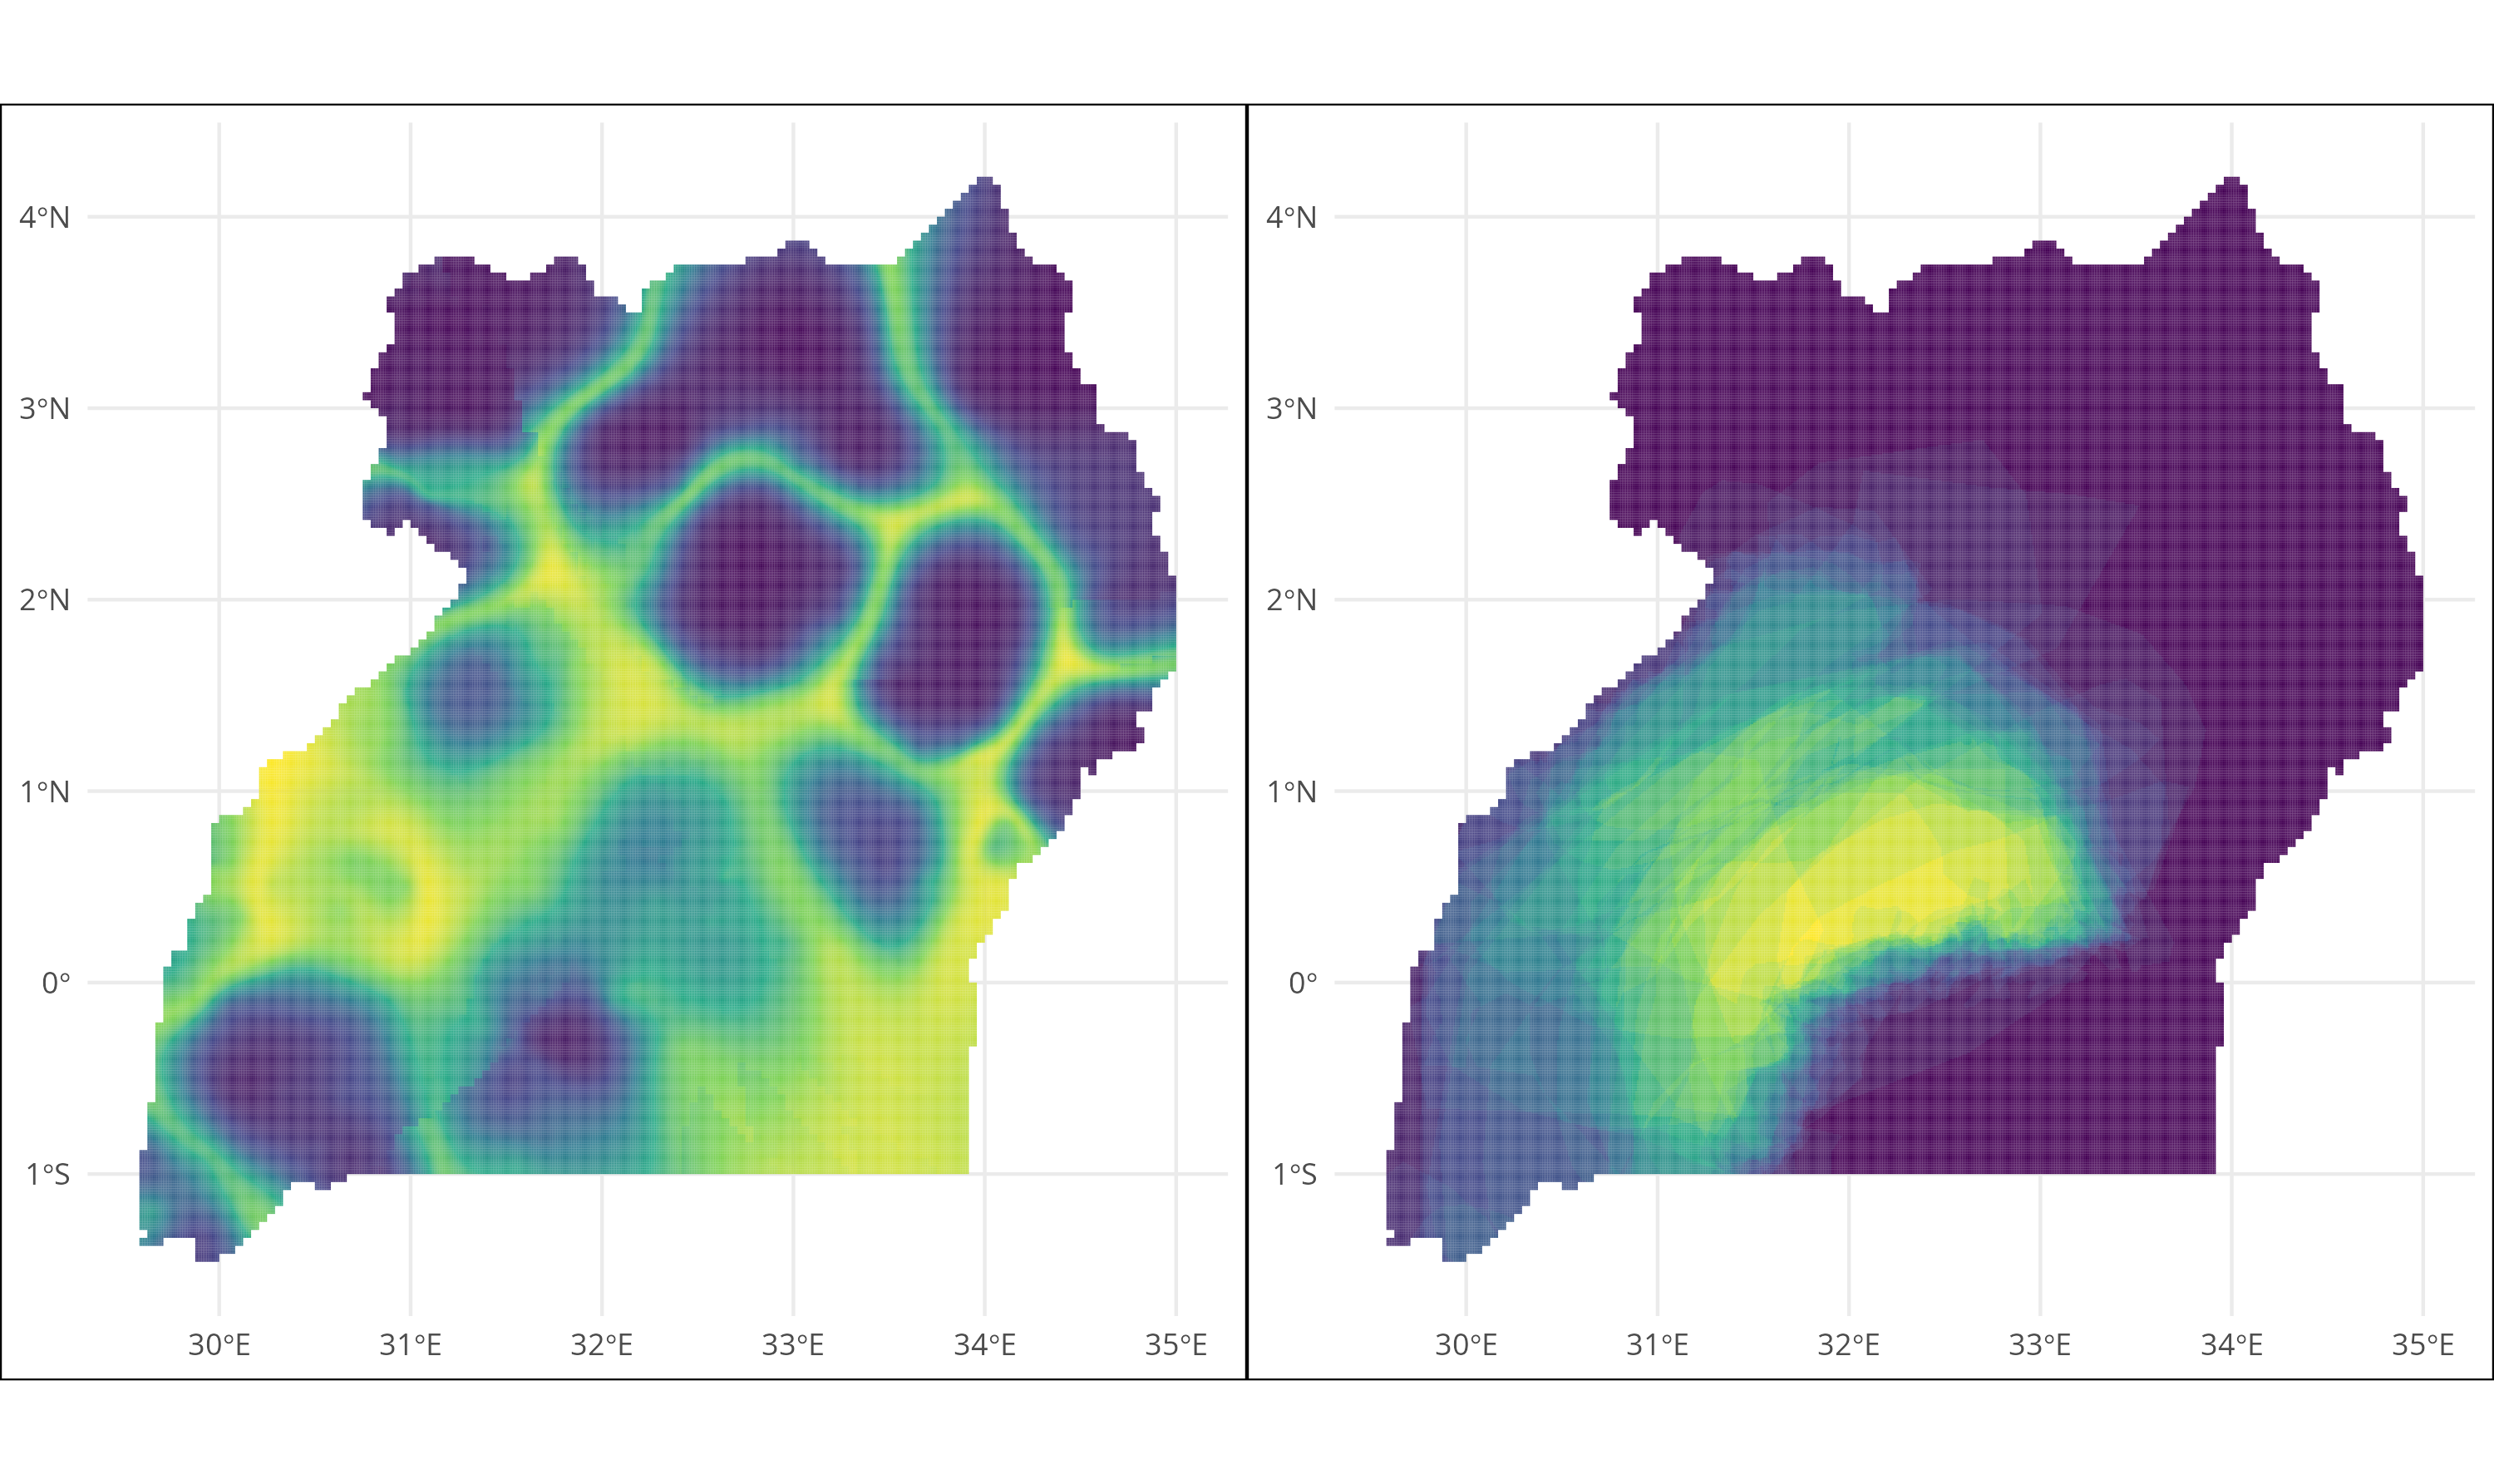
\includegraphics[width=1\linewidth]{img/ugaplots.png}
	\caption{Ethnic fractionalization (left) and state presence (right) in
	Uganda}
	\label{ugaplots}
\end{figure}

Nigeria is less clear cut, as most of the country is relatively fractionalized.
On the one hand, the only larger area of generally high ethnic fractionalization
is in the North,  corresponding to the precolonial state of Borno and adjacent
parts of the Sokoto caliphate. On the other hand, the largest relatively
homogeneous `cell' is the Hausa ethnic group in former Sokoto. Although the
latter could be due to lower population density in North Wester Nigeria, or the
relative difference in the longevity between Sokoto and Borno. The former having
been established in 1812, and the latter having roots extending into the middle
ages. However, cell-like structures, like those in Northern Uganda, look to be
more frequent in areas of low precolonial state presence.

\begin{figure}[htpb]
	\centering
	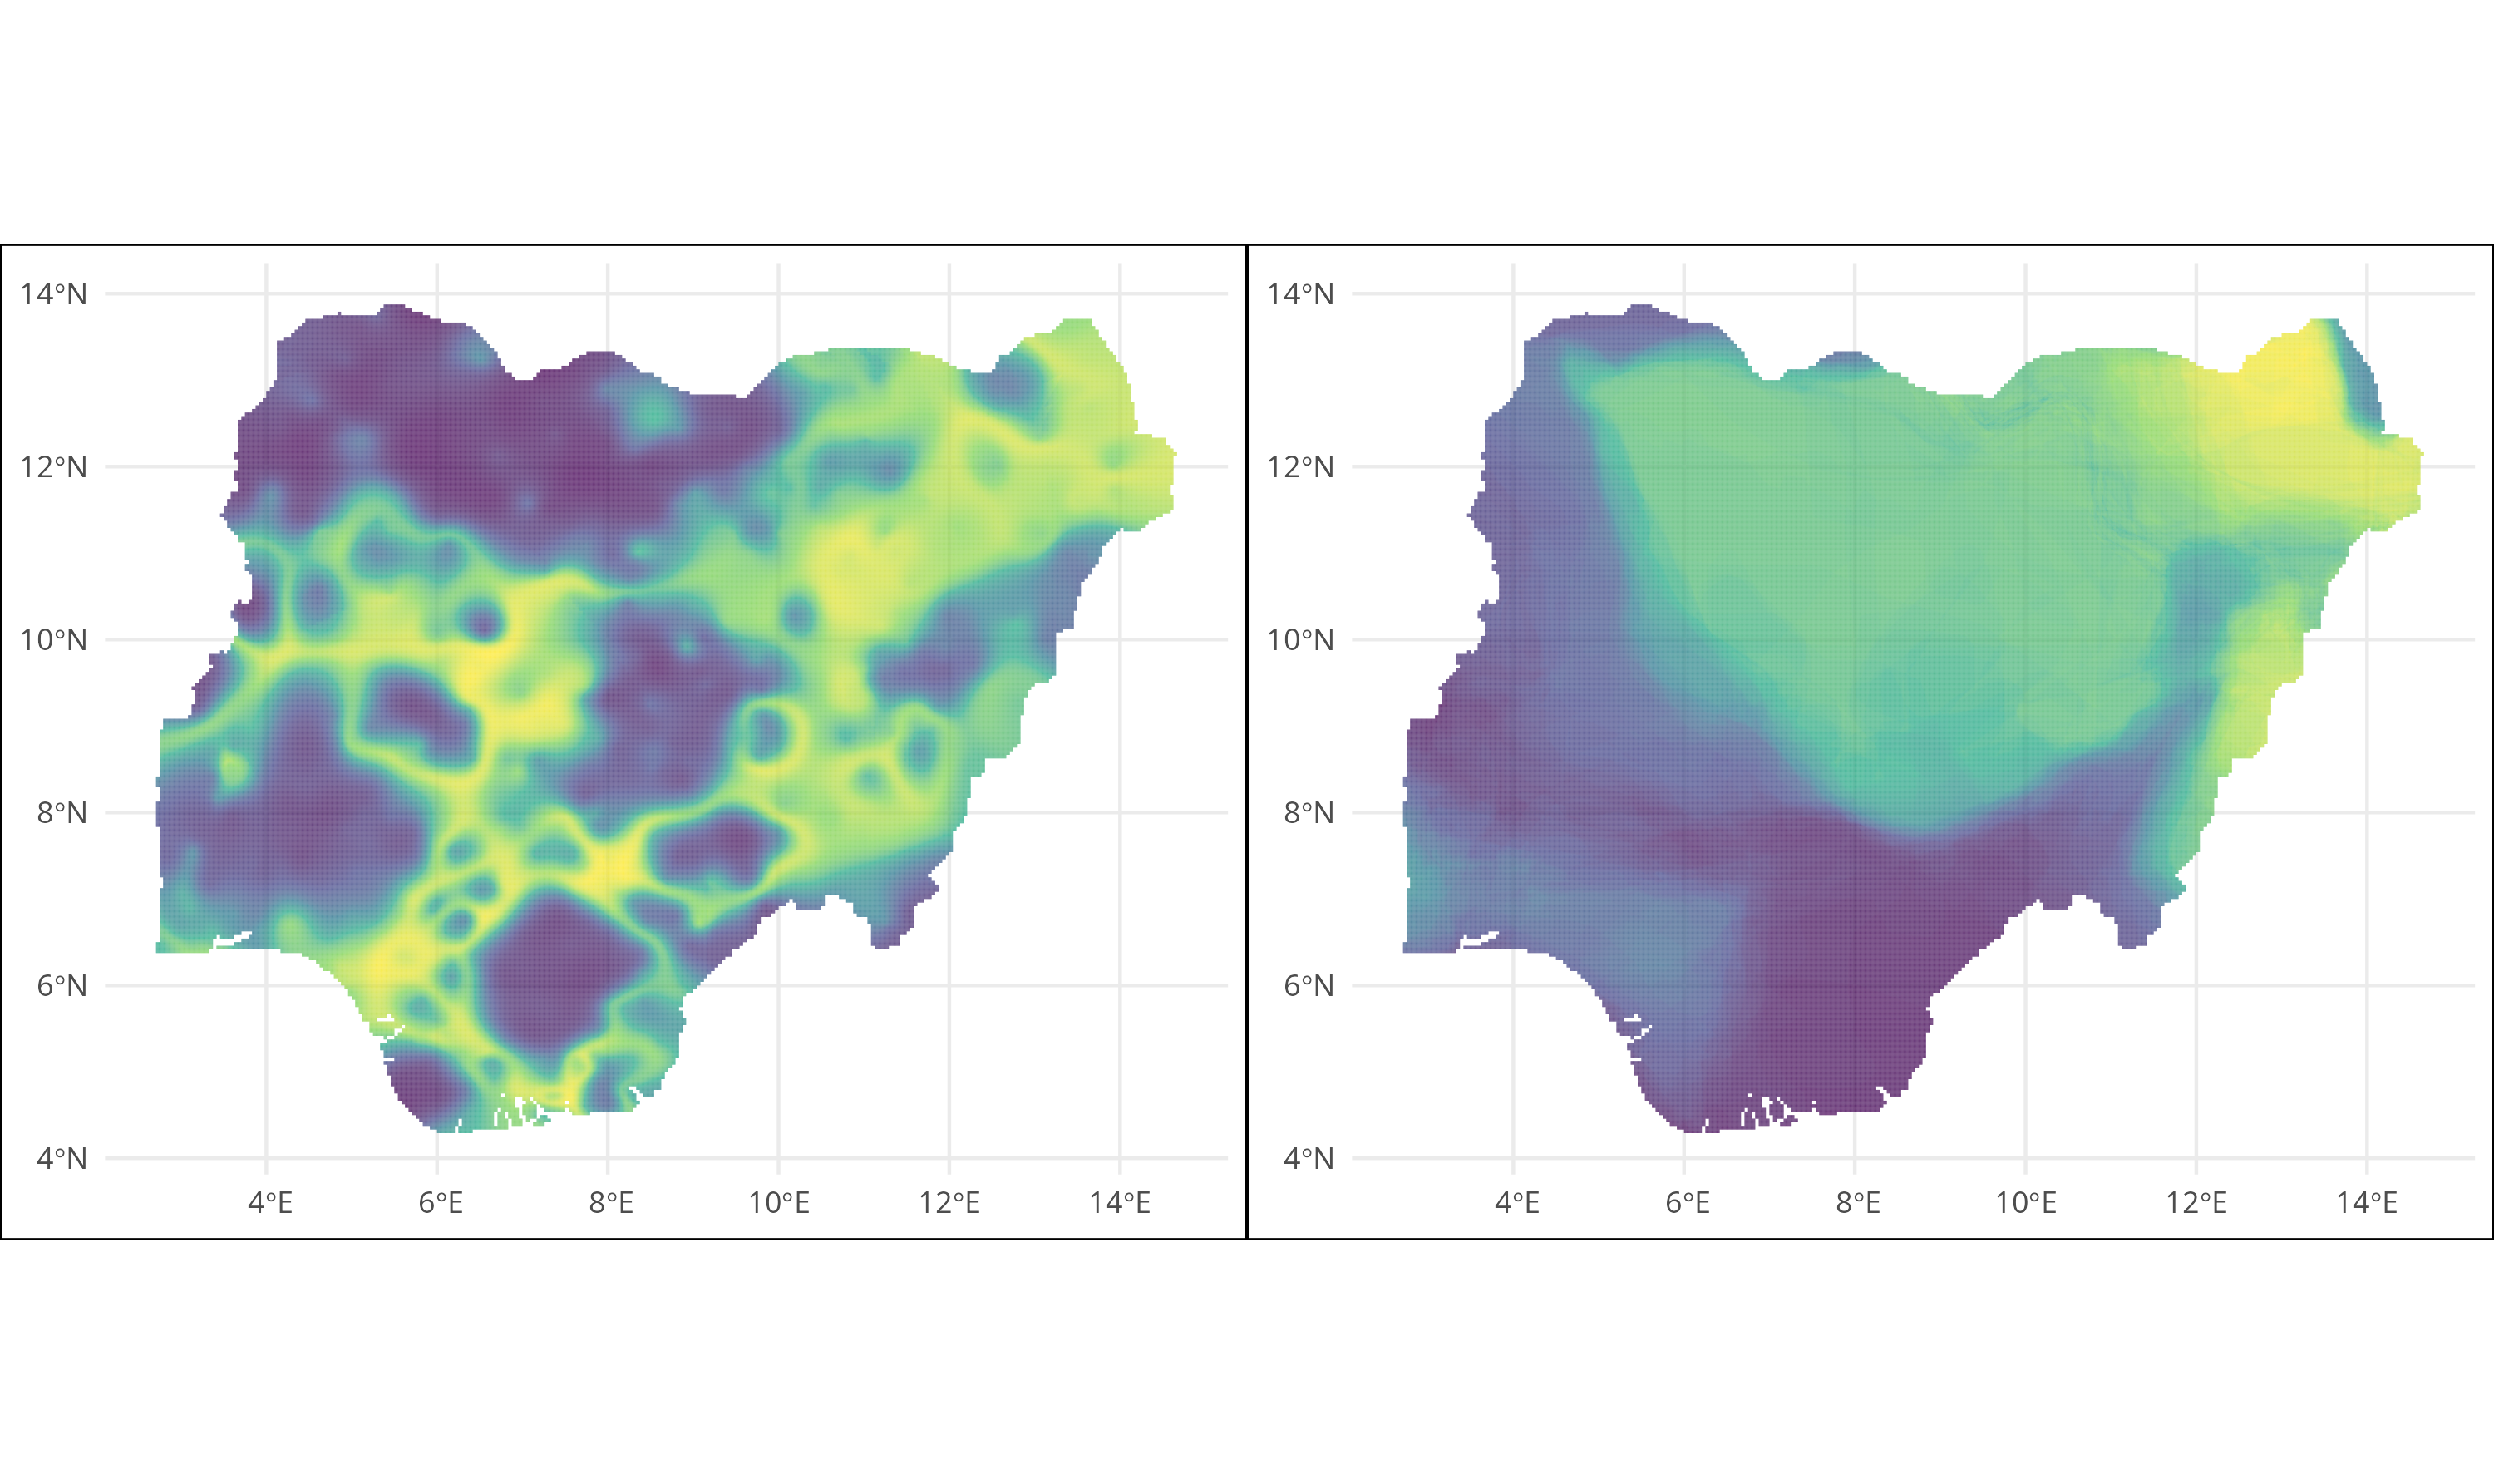
\includegraphics[width=1\linewidth]{img/nigplots.png}
	\caption{Ethnic fractionalization (left) and state presence (right) in
	Nigeria}%
	\label{nigplots}
\end{figure}

In Ghana the most ethnically diverse region seems to be on the northern
outskirts of the Ashanti kingdom, and around Accra. Again, settlement patterns
generally appear to be more cell-like in areas with low precolonial state
presence. It is also worth noting that the Ashanti ethnic group, while clearly
dominant in the core Ashanti state area is less homogeneous than some of the
larger (in terms of area) groups in the North, or the Ewe to the South East.

\begin{figure}[htpb]
	\centering
	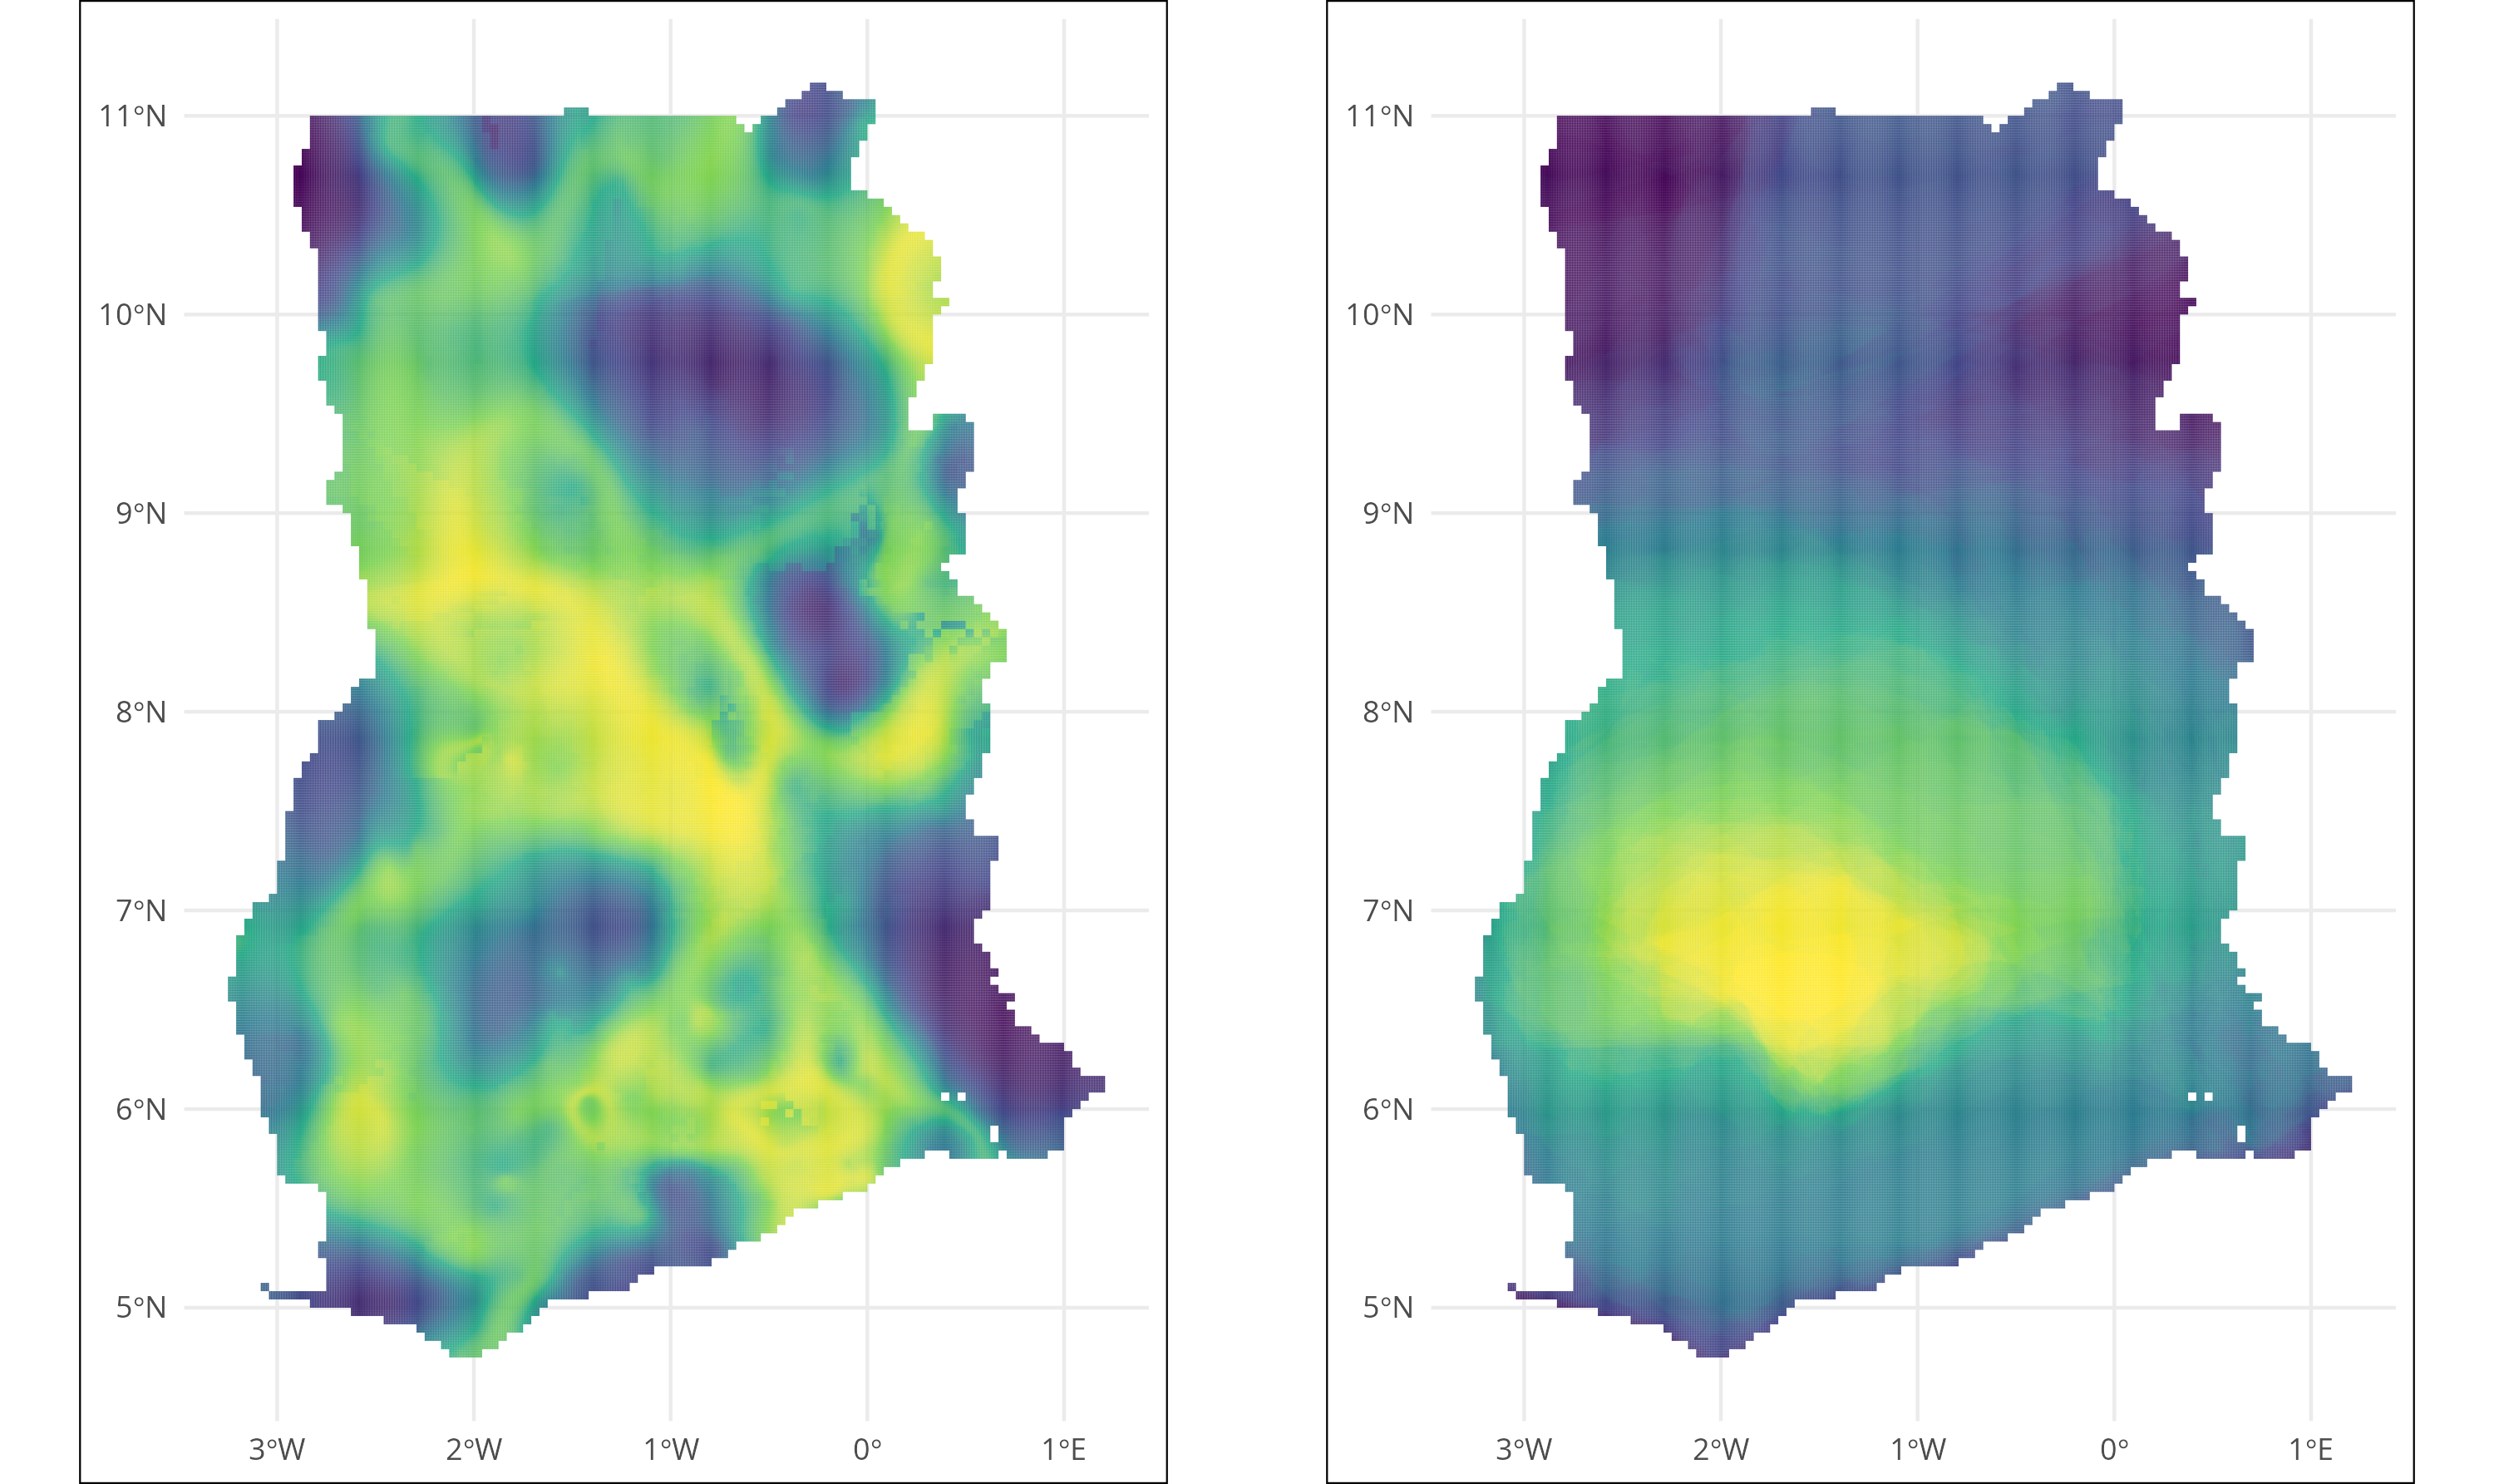
\includegraphics[width=1\linewidth]{img/ghaplots.png}
	\caption{Ethnic fractionalization (left) and state presence (right) in
	Ghana}%
	\label{ghaplots}
\end{figure}

In line with our expectations, low state presence Kenya exhibits a high degree
of cell-like settlement patterns. The exceptions being around the capital of
Nairobi and a few other smaller pockets.\footnote{At least one of which is the
	Chalbi desert in the North, which has little to no population. This
	makes the fractionalization measure sensitive to swinging to either
extreme, especially given SIDE's method for interpolating data it seems (ref.
Lake Victoria).} The area along the South East coast had some state presence
from the Zanzibar sultanate, but appears at first glance homogeneous like the
rest of Kenya. However, at least two coastal cities stand out. This is not
surprising both because they are cities, and because the Zanzibar sultanate was
a coastal trading state, whose control seldom extended beyond fortified coastal
cities. Thus, the maps on which our data on state presence is based, has a
tendency of overstating the size of the sultanate.

\begin{figure}[htpb]
	\centering
	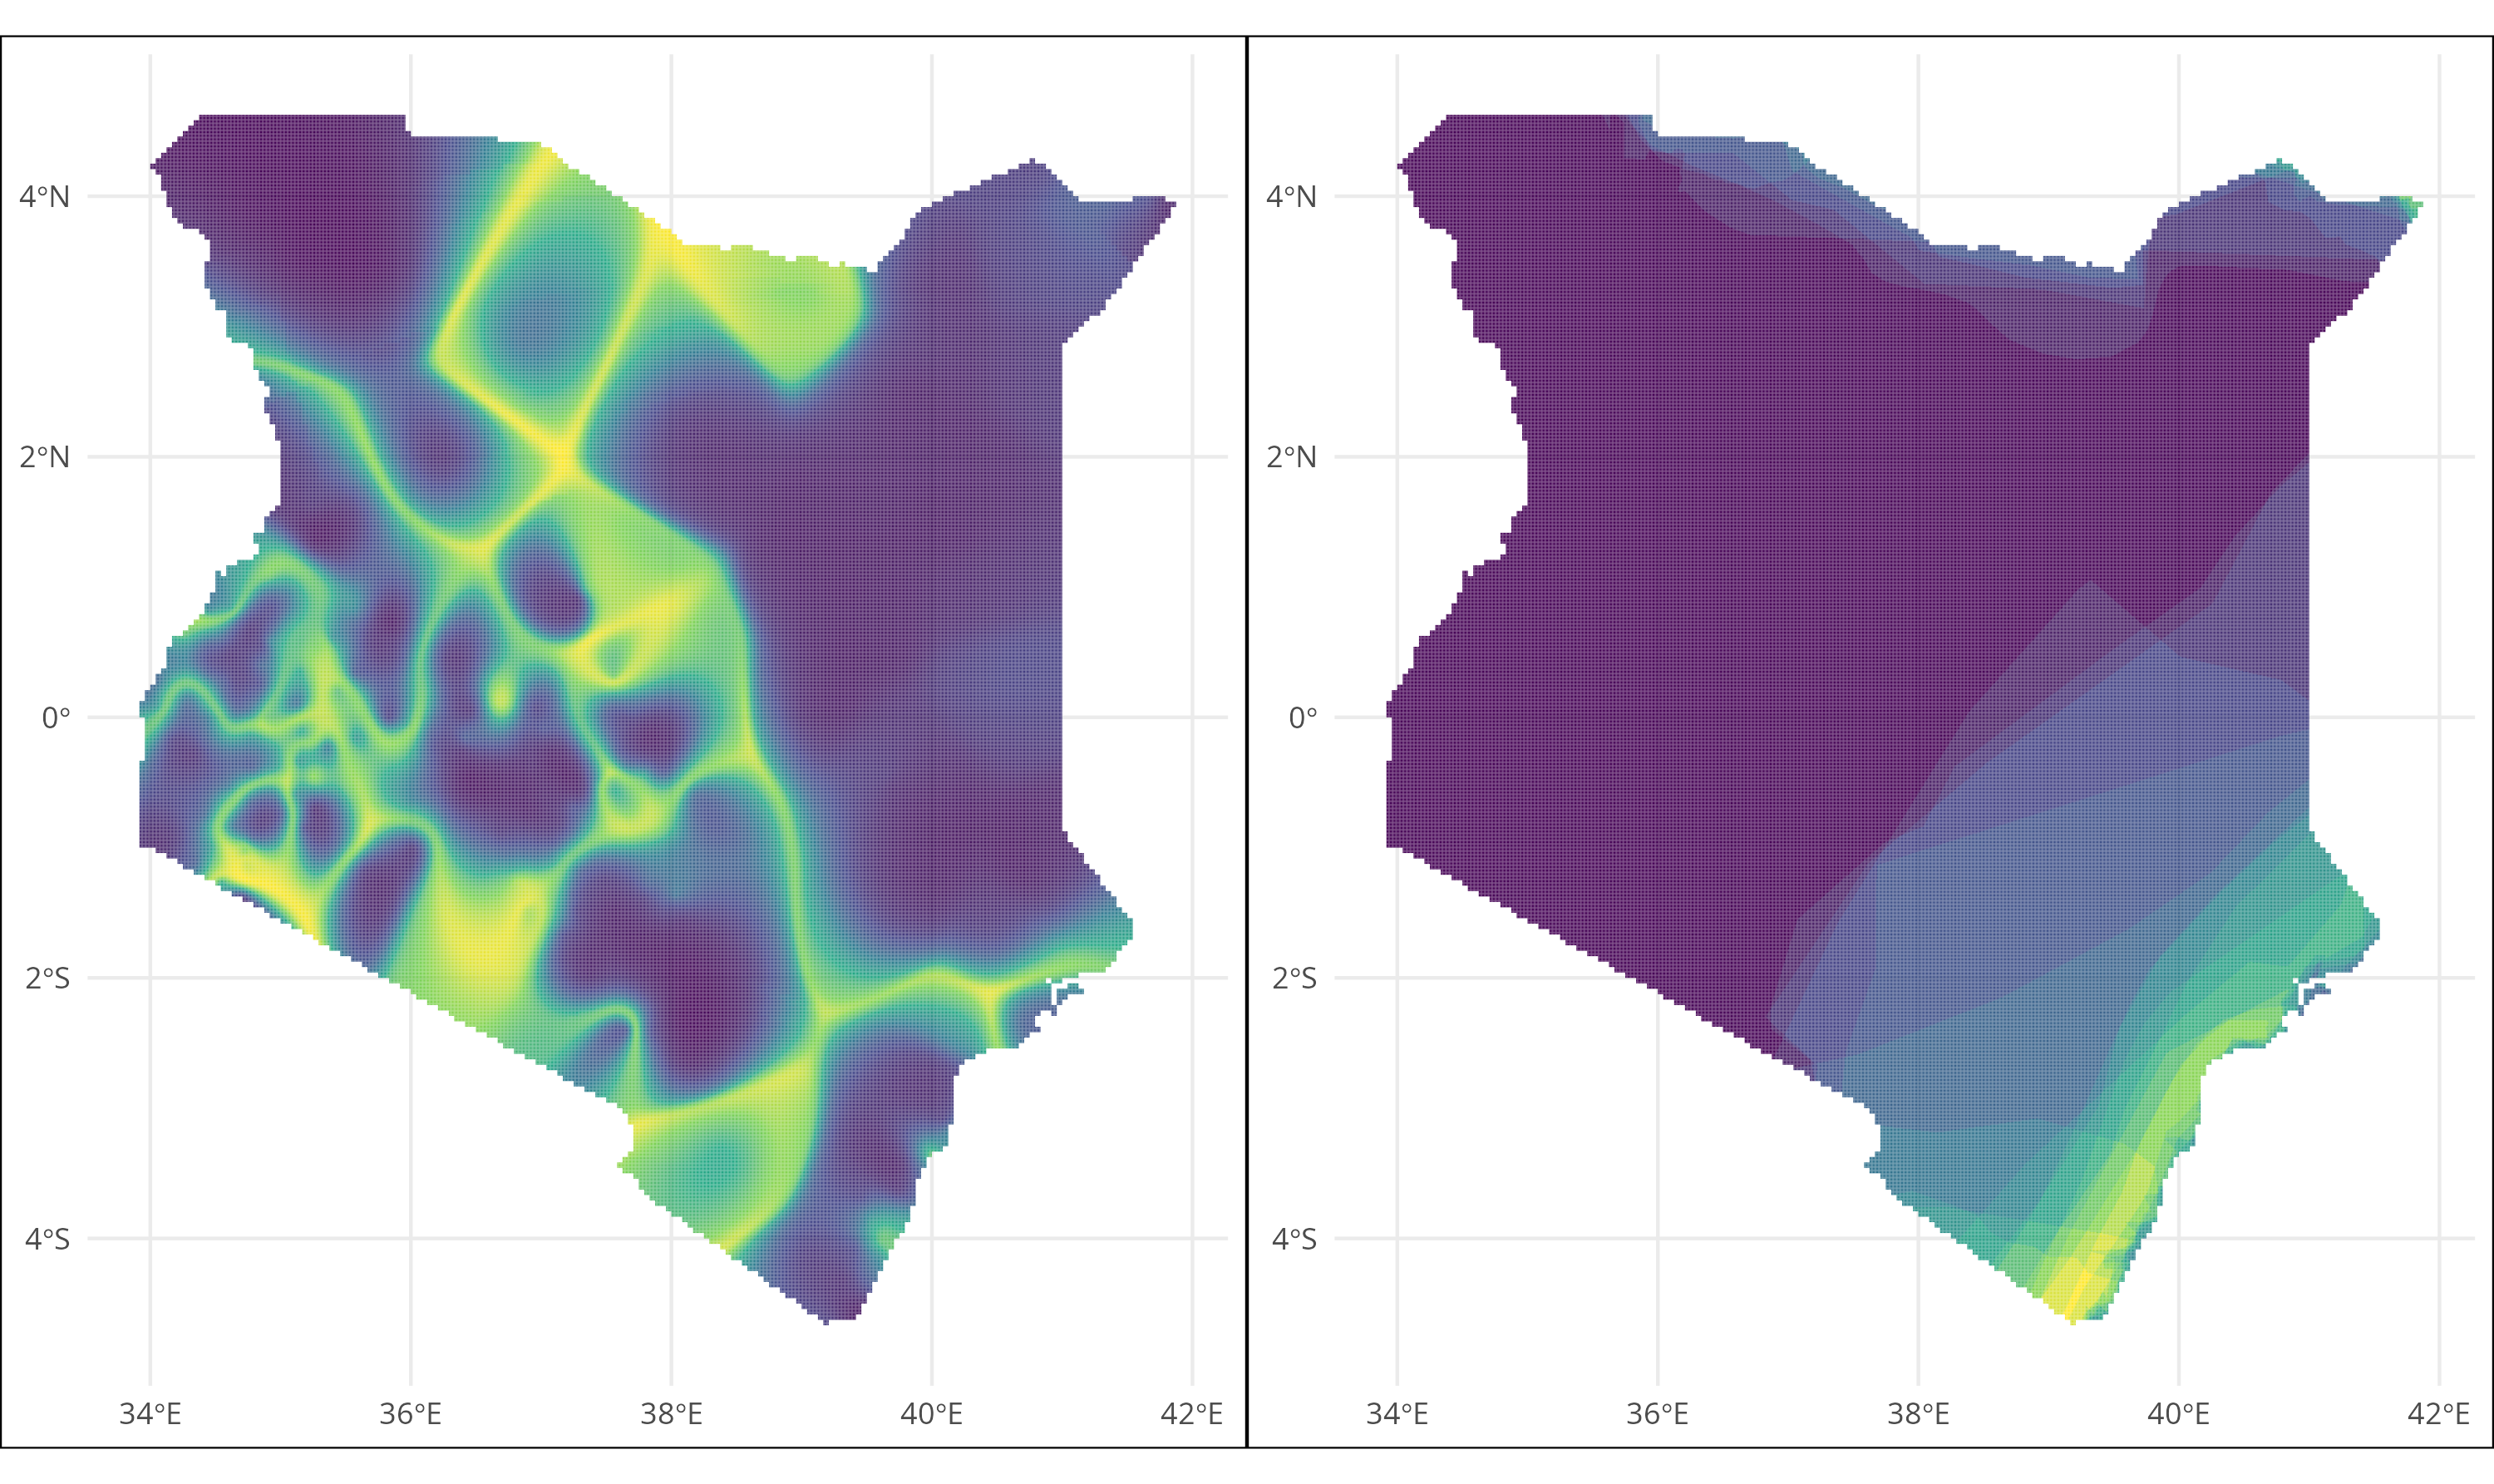
\includegraphics[width=1\linewidth]{img/kenplots.png}
	\caption{Ethnic fractionalization (left) and state presence (right) in
	Kenya}%
	\label{kenplots}
\end{figure}

Overall, the evidence on settlement patterns indicate that Precolonial states
have allowed for more inter-group interaction and greater ethnic
fractionalization -- presumably by setting in motion the virtuous cycle sketched
out in Figure \ref{causal}.

\section{Conclusion} \label{Conclusion}

This article combines the literature on states' efforts to limit inter-group
violence in their territory \citep{Olson1993, Pinker2012, tilly_1985}, with
literature arguing that for many places in Africa the precolonial topography of
state presence, or lack thereof, has been surprisingly
persistent \citep{boone2014property, englebert2013inside}. We argue that this
suggests that areas with more precolonial experience of statehood started the
post independence period with lower rates of communal violence. The precolonial
states initially provided institutions designed to solve the commitment problem,
and by acting as an overarching arbiter helped reduce the security dilemma. This
set in motion a positive feedback loop whereby increased trade -- and thereby
interactions -- which simultaneously increased relative costs of violence,
reduced the information problem and led to less effective anonymity towards
non-coethnics, which reduced the risk of individual cheaters. The cost saving
prerogatives of colonizers, and the weakness of the post independent states
meant that many of these institutions and relationships often survived at the
local level, which has allowed the initial difference in local levels of
communal violence to persist. 

Using new data on precolonial statehood, we find evidence of a general effect of
precolonial state presence on local levels of communal violence. This effect is
particularly pronounced in East Africa, but appears to be sensitive to
measurement of the dependent variable in West-Africa. We also find some evidence
that ethnic settlement patters could be driven, in part, by precolonial states'
ability to suppress inter-group violence. 


\clearpage

\bibliographystyle{apsr}
\bibliography{../lib.bib}

\clearpage

\section{Appendix} \label{Appendix}

\import{../R/Output/}{CVsummaryStats.tex}

\begin{sidewaysfigure}[htpb]
	\centering
	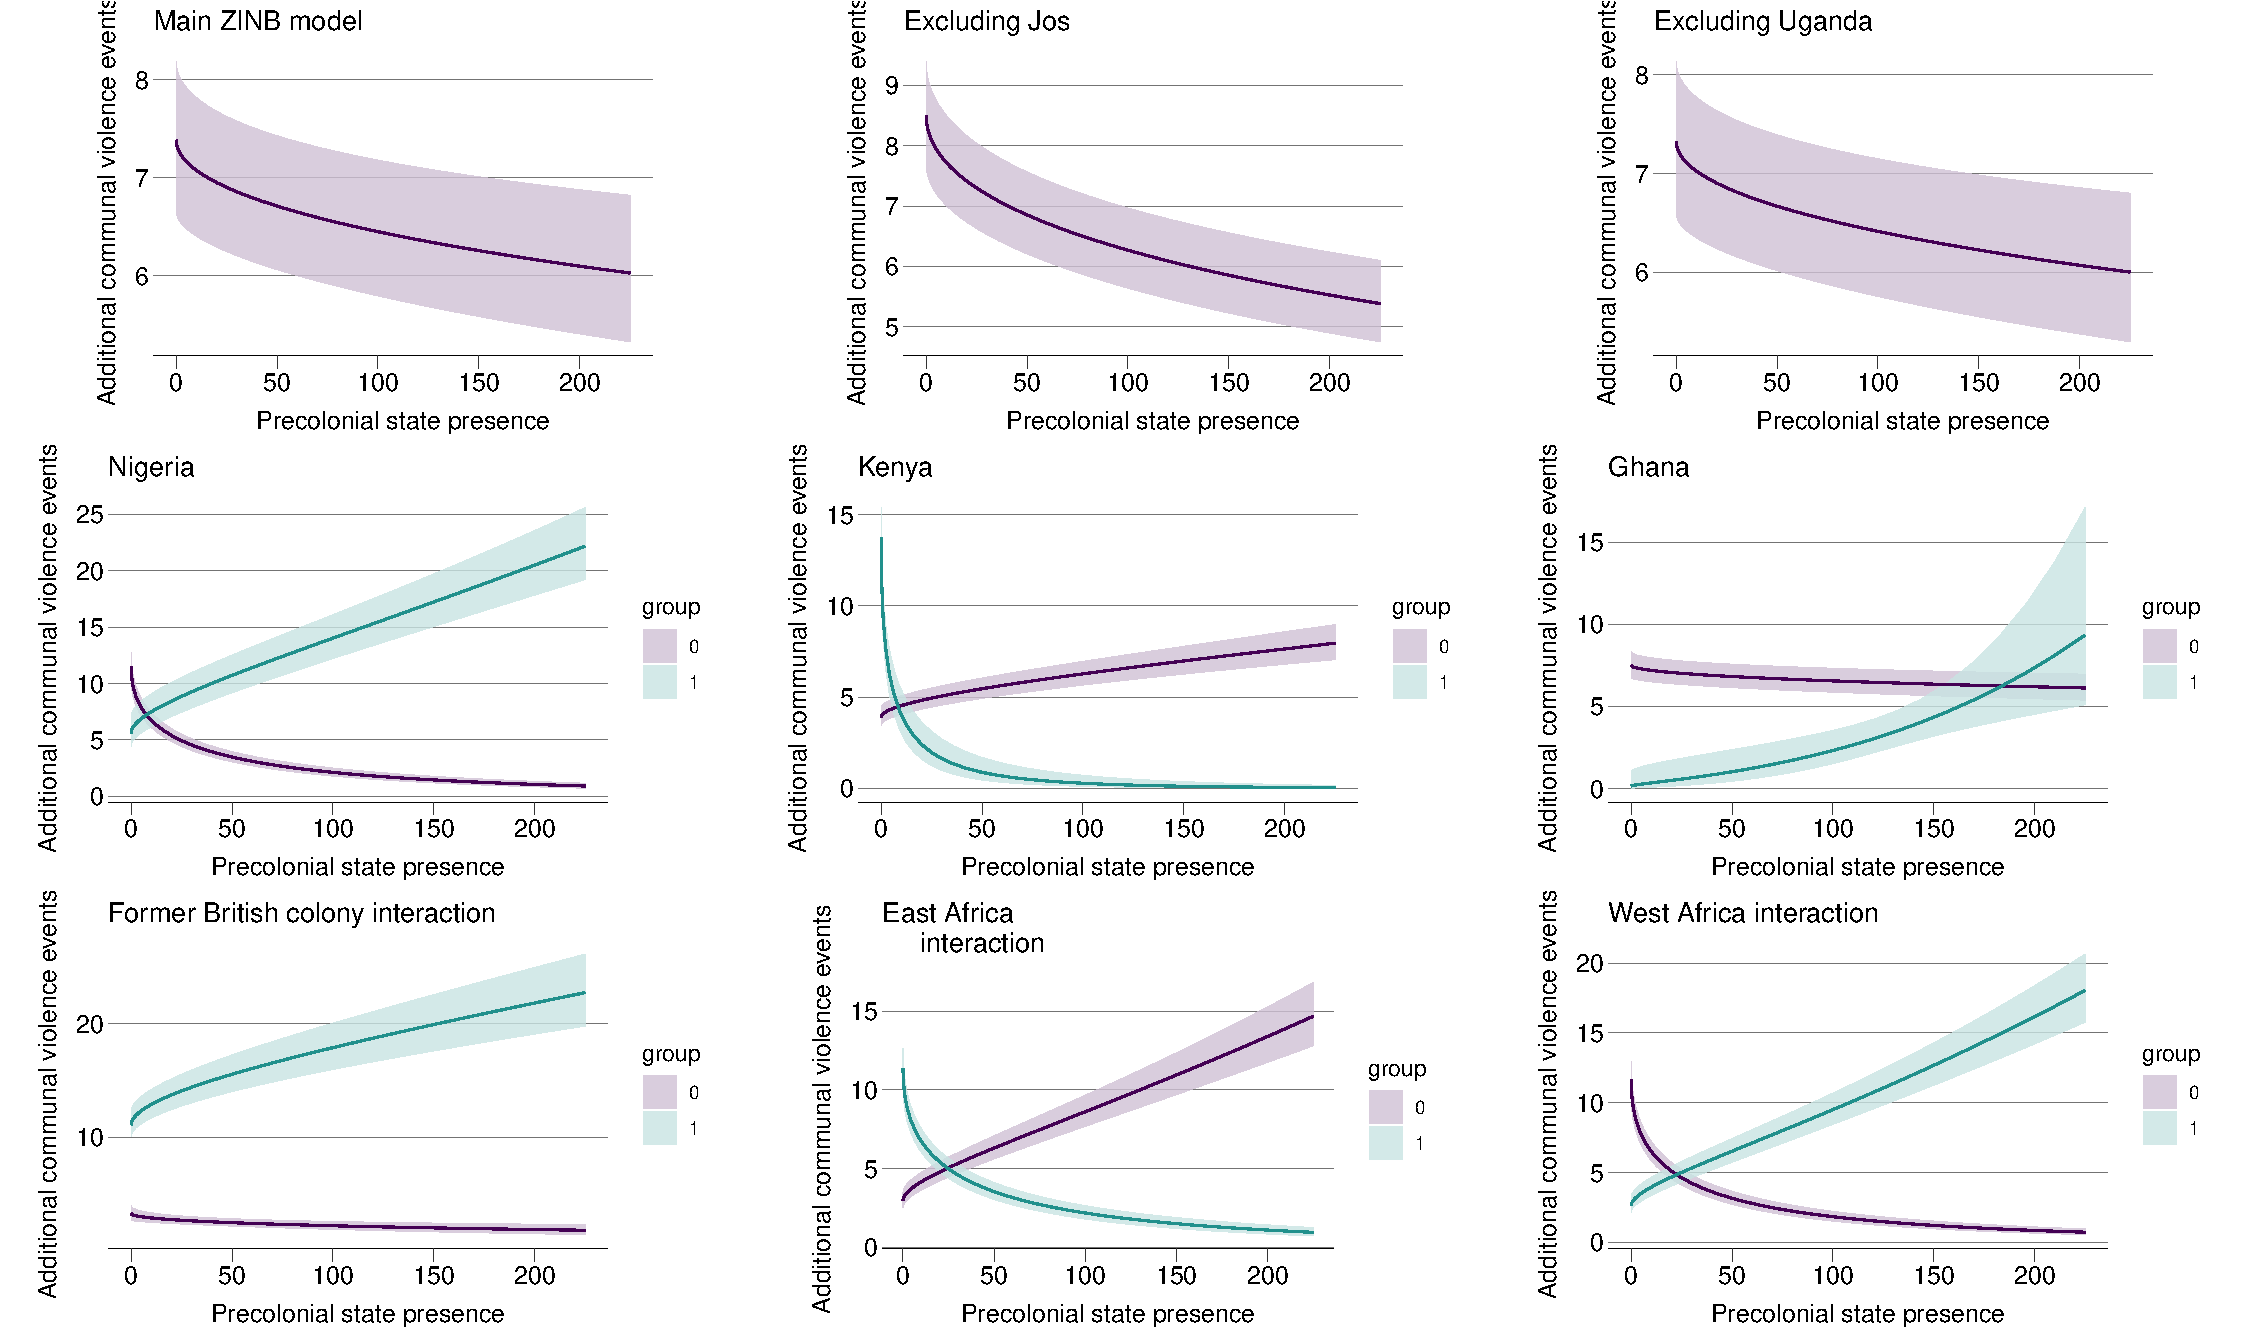
\includegraphics[width=1\linewidth]{R/Output/org3plots.pdf}
	\caption{Communal violence ZINB-count models}
	\label{org3plots}
\end{sidewaysfigure}

\begin{sidewaysfigure}[htpb]
	\centering
	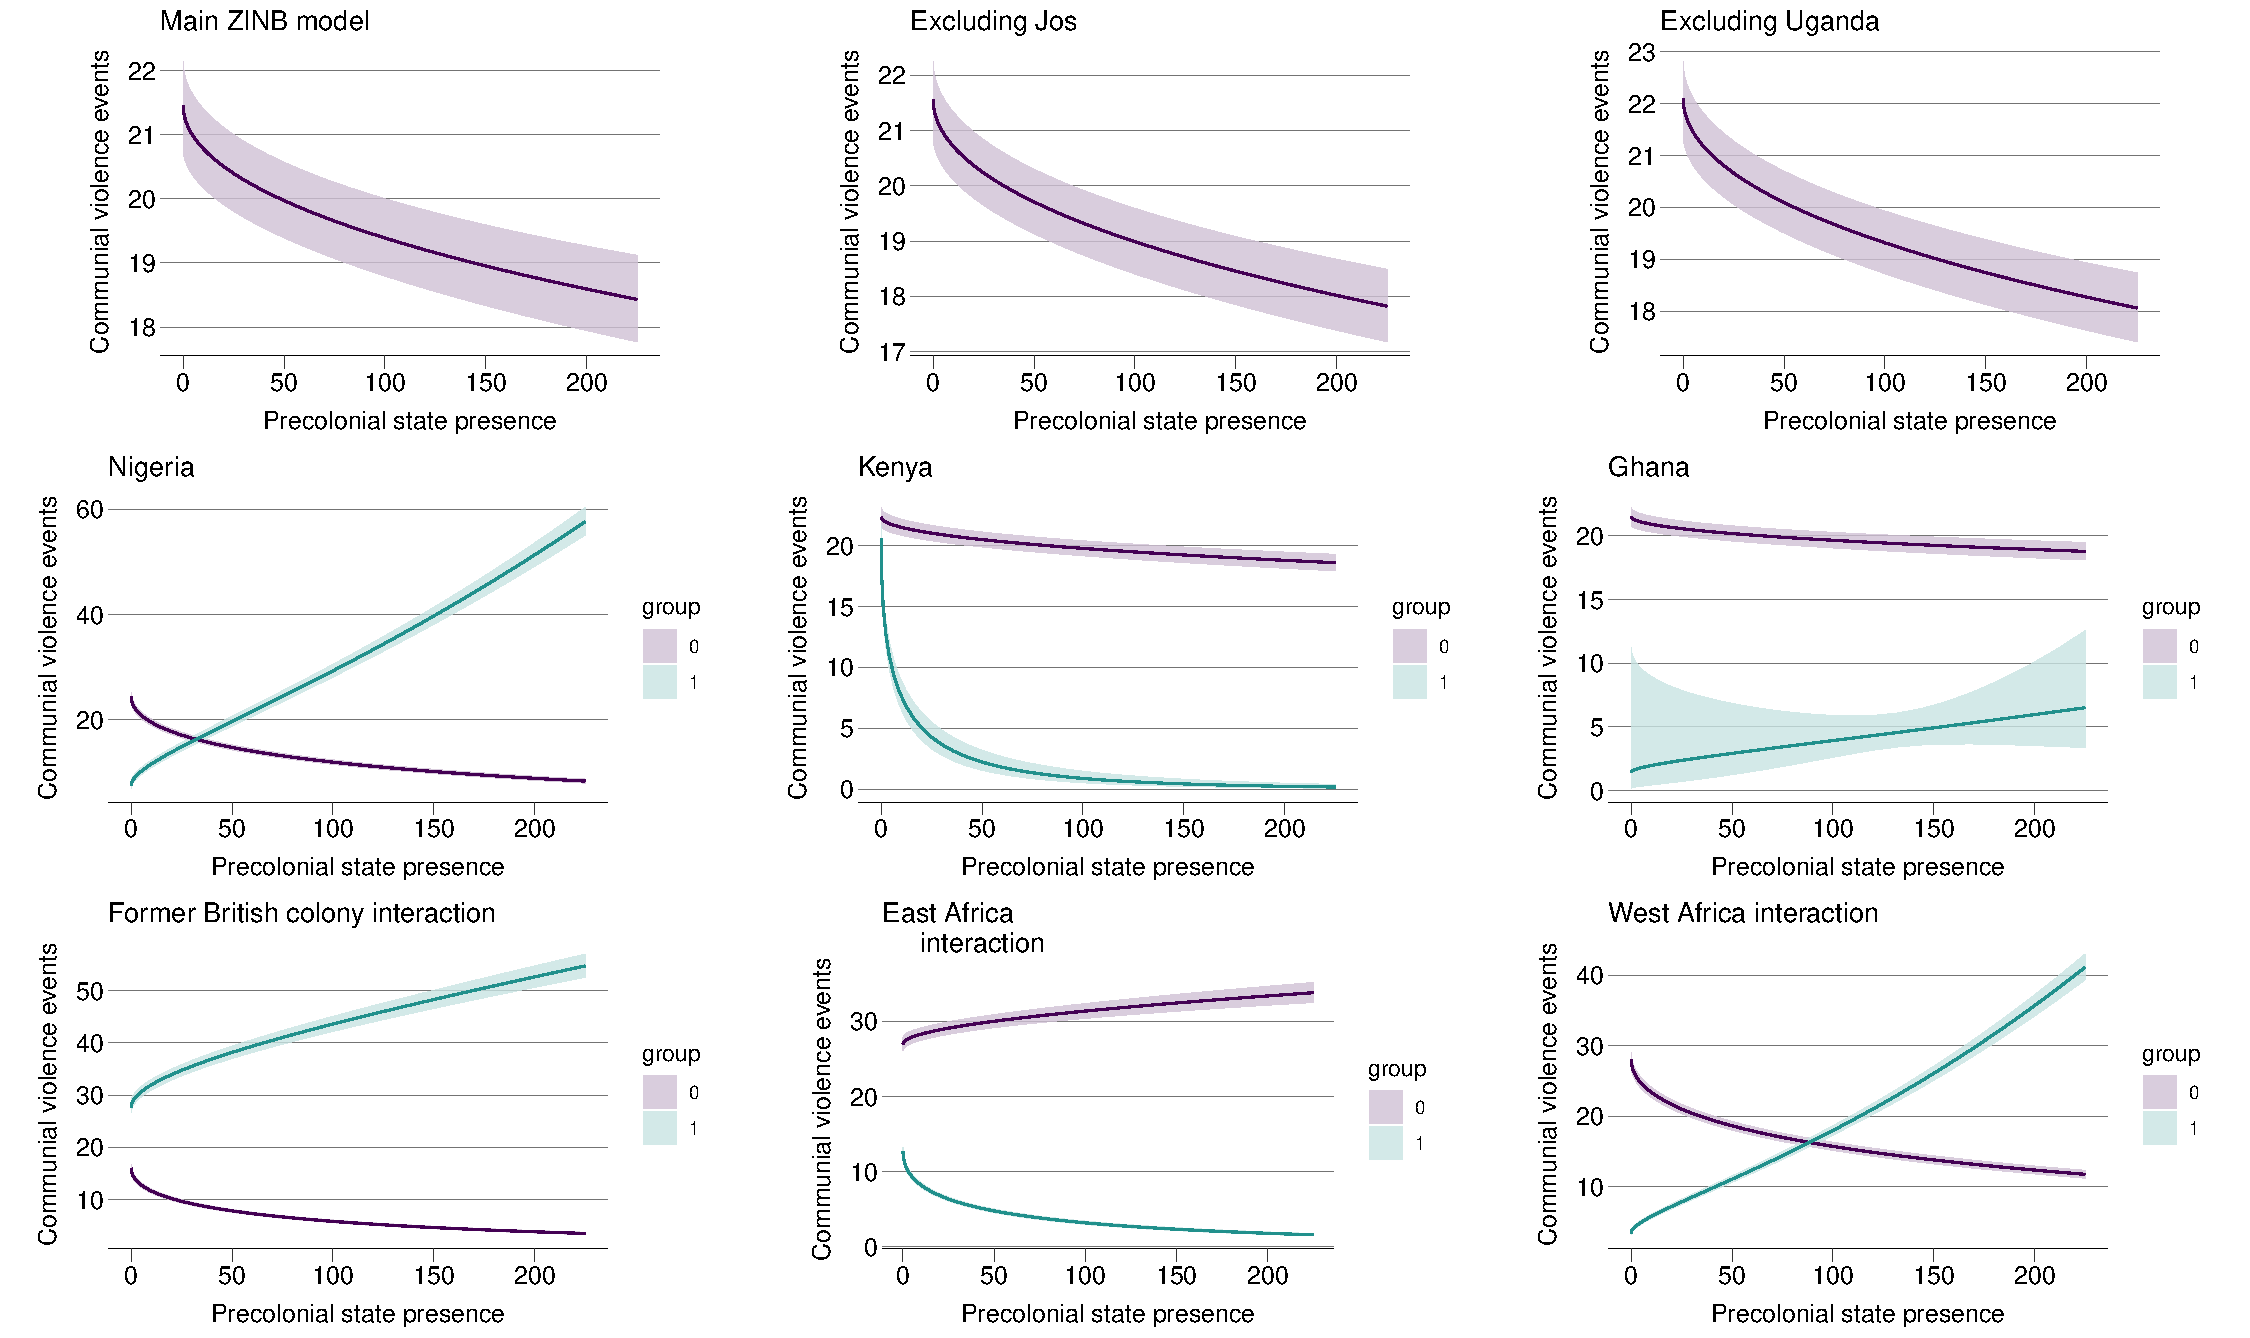
\includegraphics[width=1\linewidth]{R/Output/nonstateplots.pdf}
	\caption{Non-state violence ZINB-count models}
	\label{non-stateplots}
\end{sidewaysfigure}

\begin{sidewaysfigure}[htpb]
	\centering
	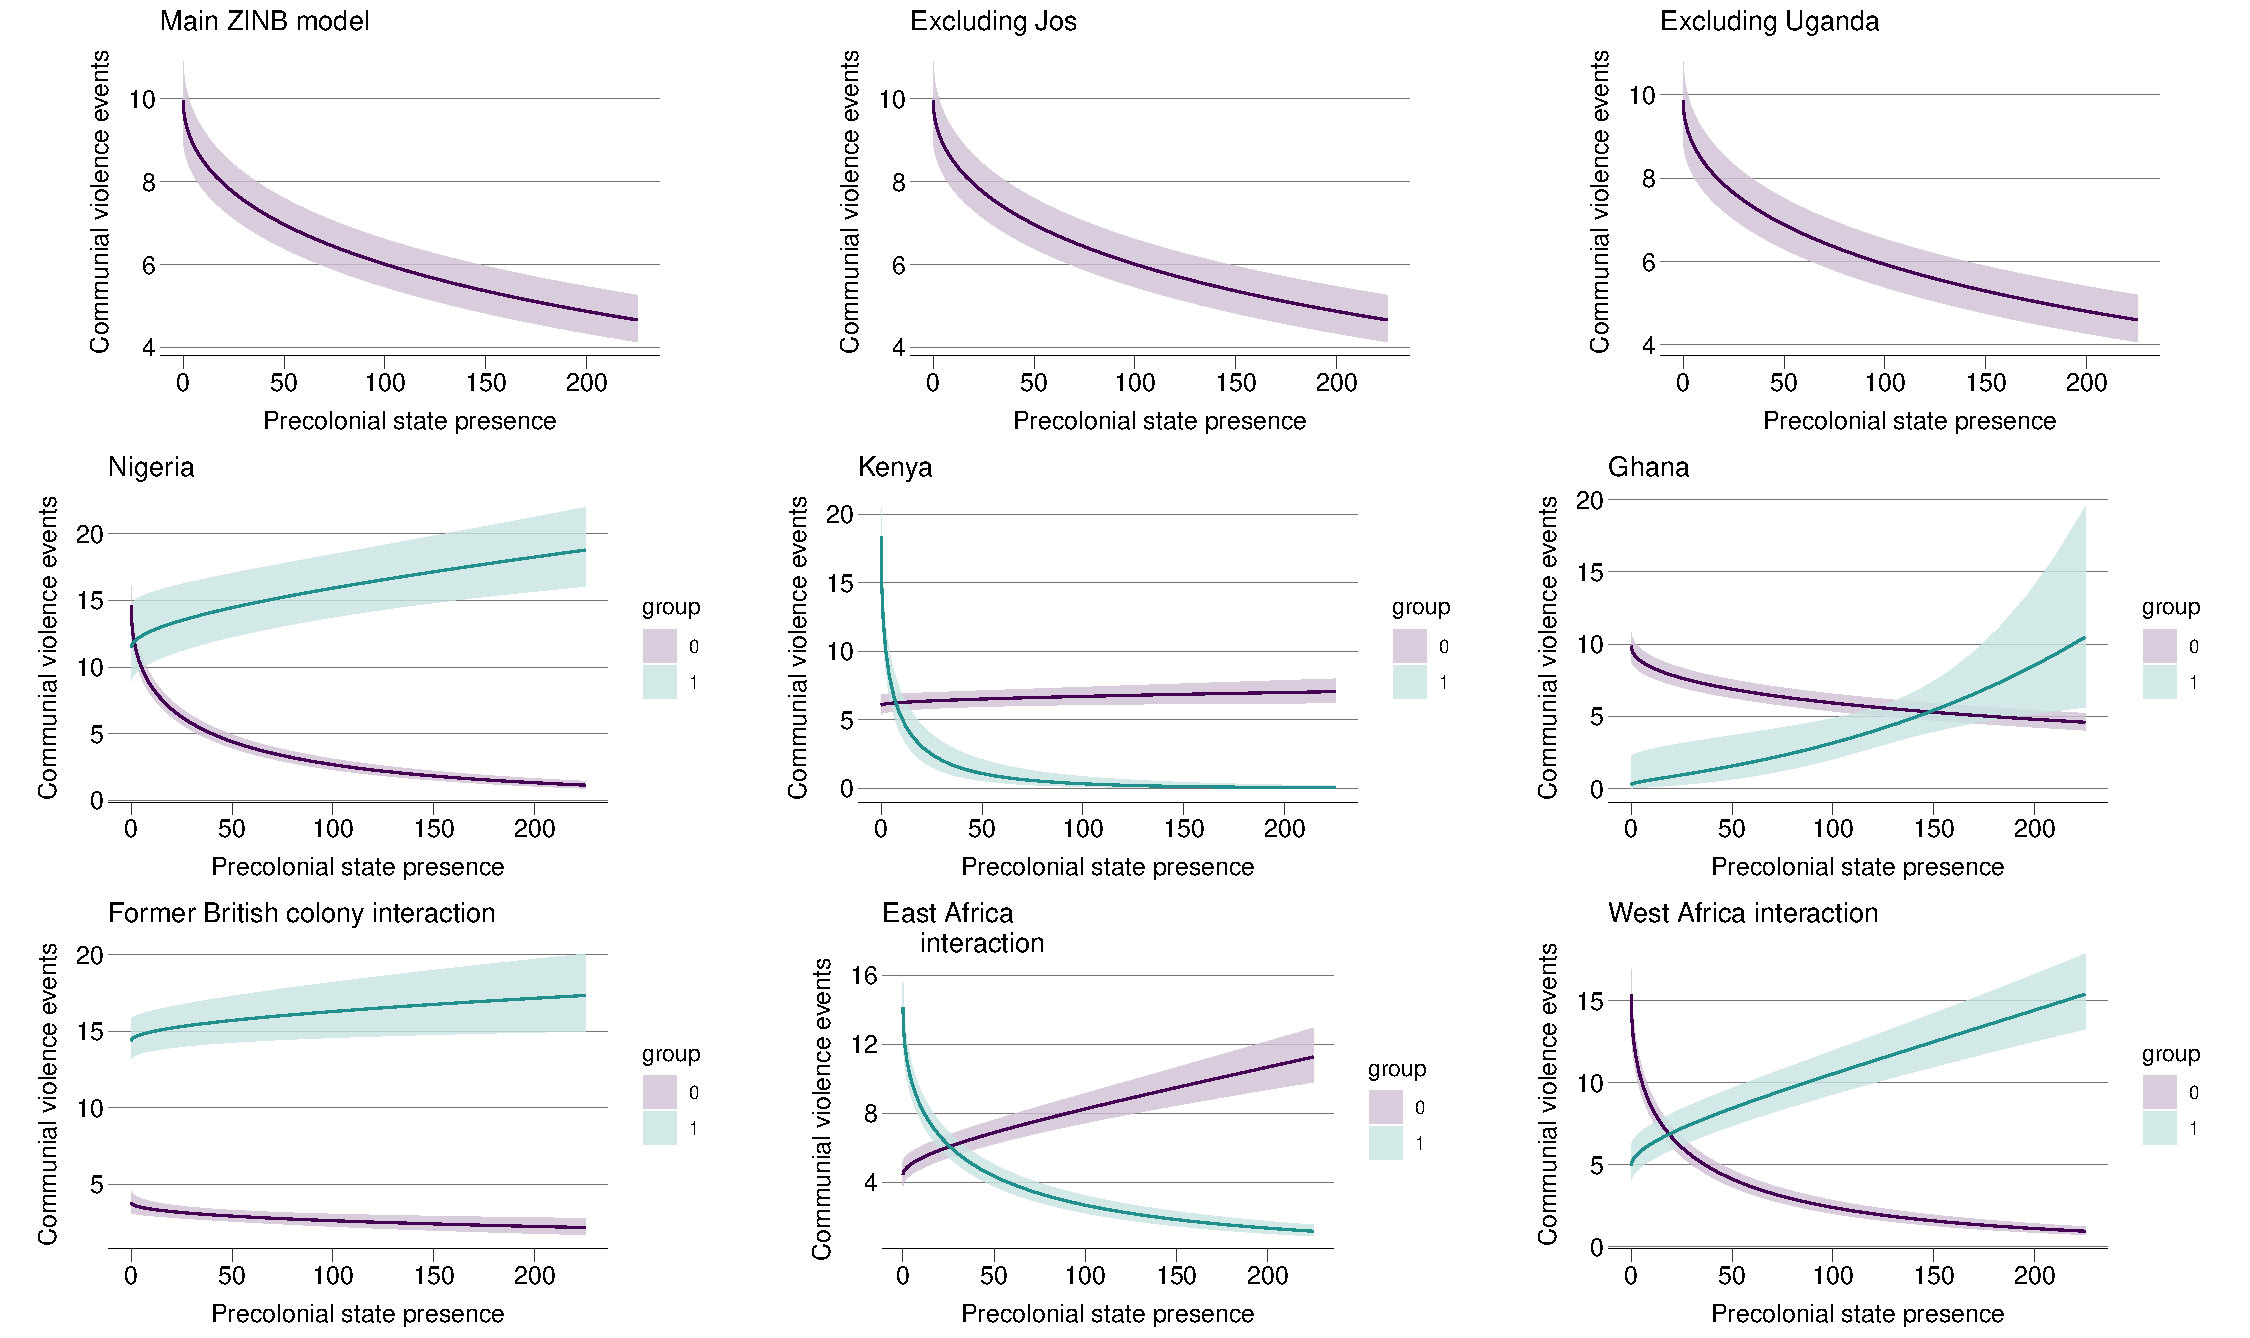
\includegraphics[width=1\linewidth]{R/Output/noreligioninnigplots.pdf}
	\caption{Communal violence ZINB-count models (excluding Christian-Muslim
	dyad in Nigeria)}
	\label{noreligion}
\end{sidewaysfigure}

\begin{sidewaysfigure}[htpb]
	\centering
	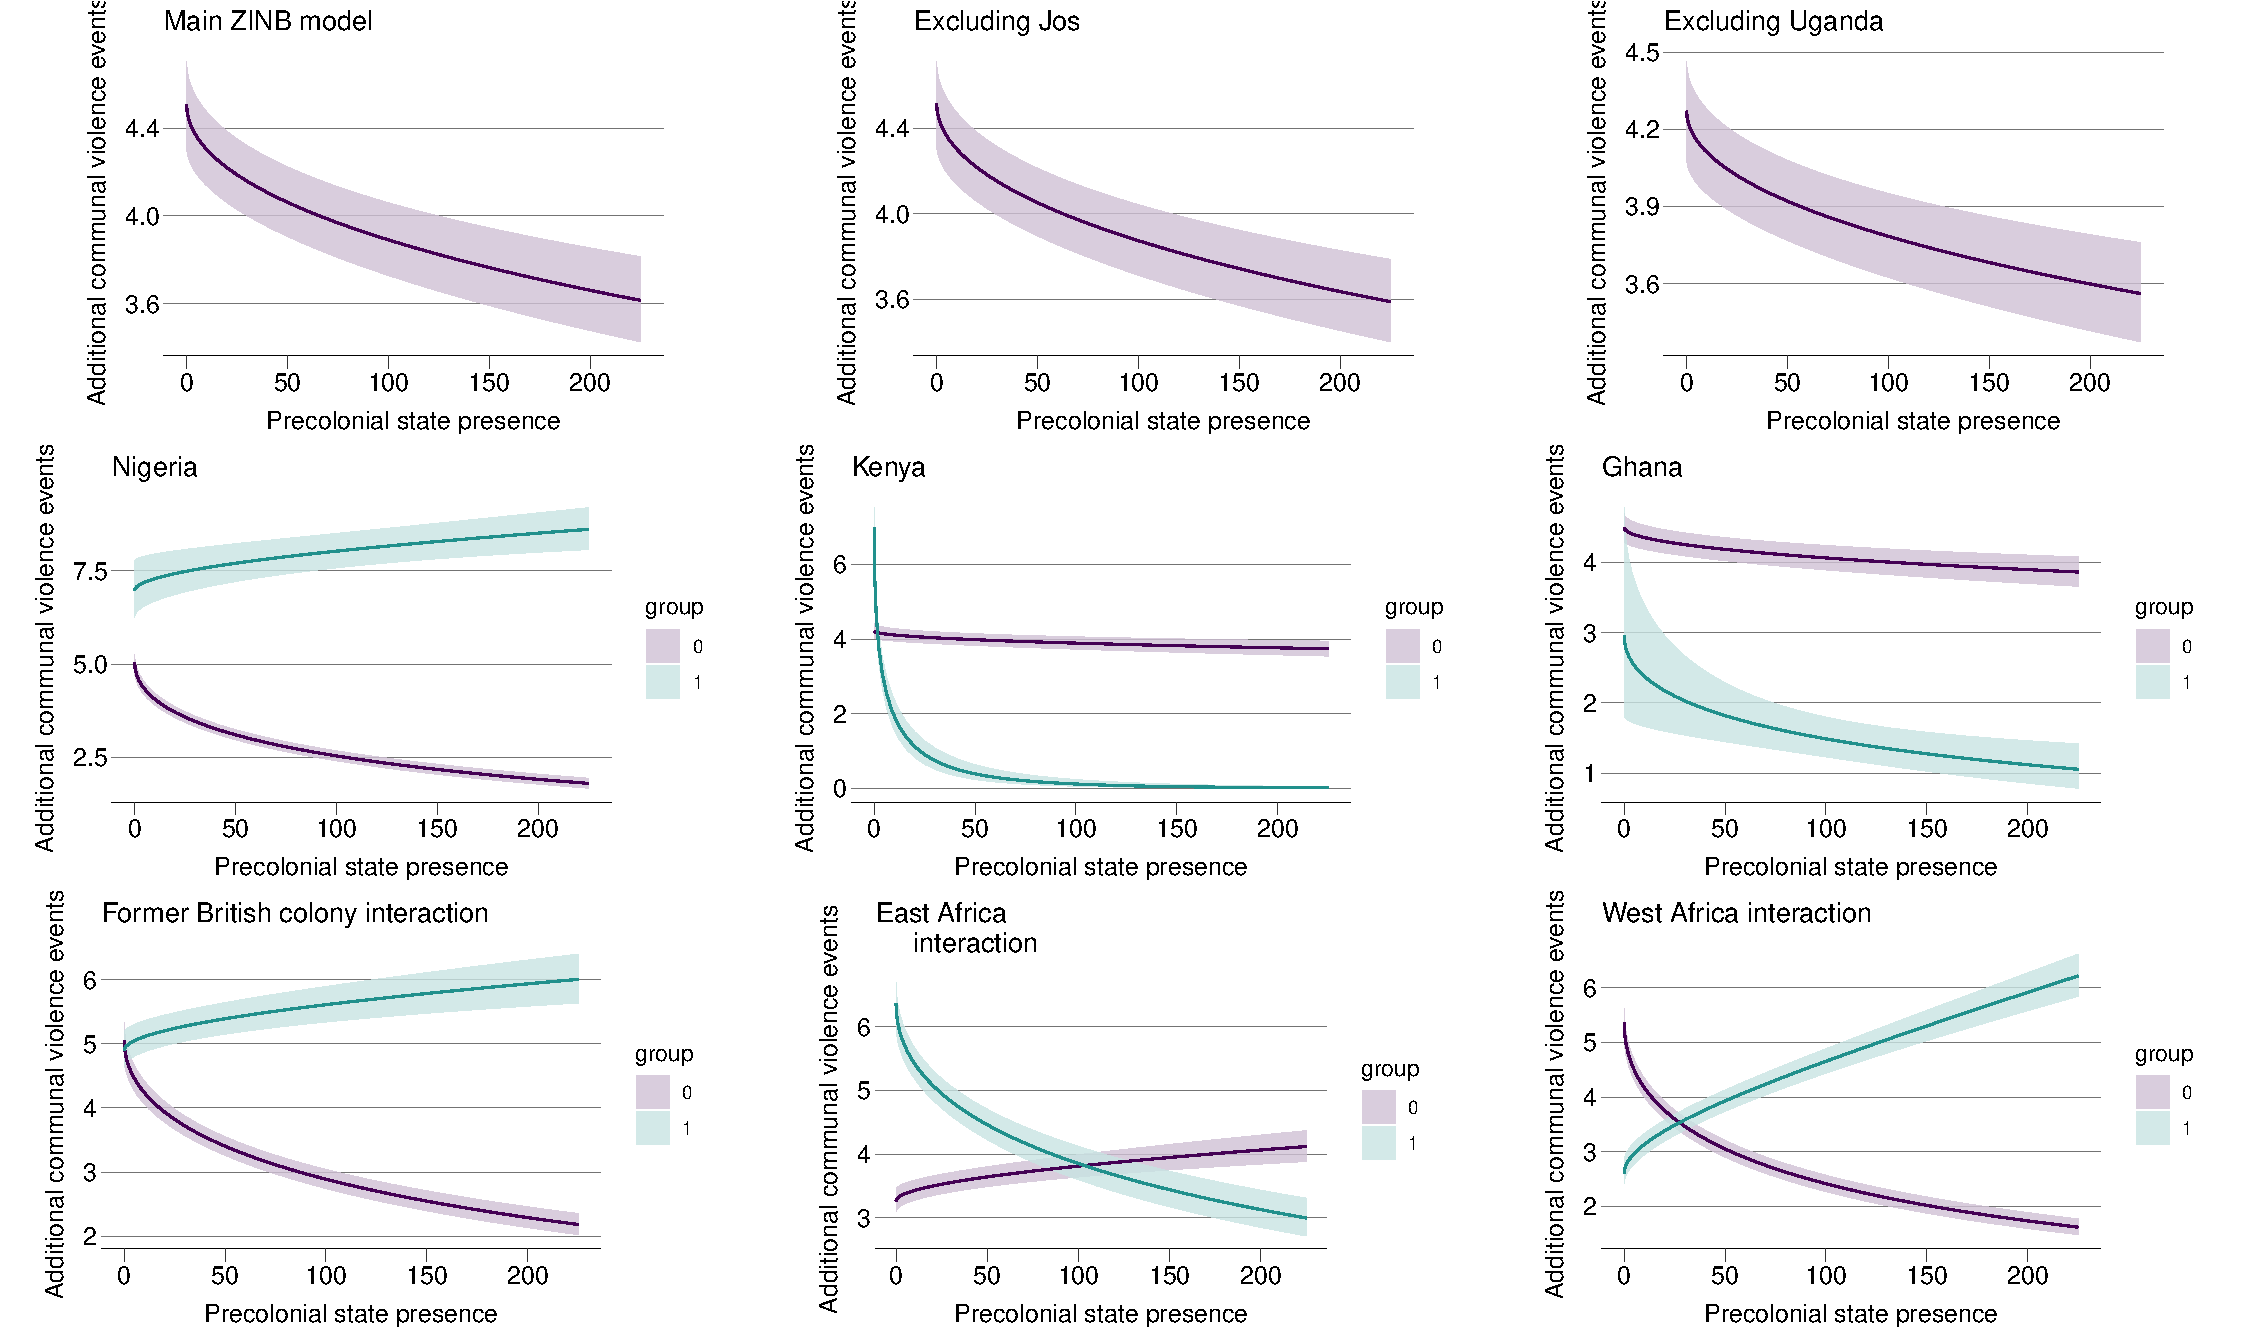
\includegraphics[width=1\linewidth]{R/Output/acledplots.pdf}
	\caption{Communal violence ZINB-count models (ACLED events)}
	\label{acledplots}
\end{sidewaysfigure}

\import{../R/Output/}{org3}
\import{../R/Output/}{non_state}
\import{R/Output/}{czinborg3}
\import{R/Output/}{czinbnon_state}
\import{R/Output/}{czinbacledev}
\import{R/Output/}{zzinborg3}
\import{R/Output/}{zzinbnon_state}
\import{R/Output/}{zzinbacledev}
\import{../R/Output/}{side}

	
